\documentclass[article,final,14pt]{scrreprt}
% \documentclass[14pt,pdf,hyperref={unicode}]{beamer}
\usepackage[utf8x]{inputenc}
\usepackage[russian]{babel}
\usepackage{amsfonts}
\usepackage{enumerate}
\usepackage{amsthm}
\usepackage{amssymb}
\usepackage{vmargin}
\usepackage{amsmath}
\usepackage{graphicx}
\usepackage{listings}
\usepackage{color}
\usepackage{multicol}
\usepackage{pb-diagram}
\usepackage[Bjornstrup]{fncychap}
\usepackage{xcolor}
\usepackage{esint}
\usepackage{tocloft}
\usepackage{hyperref}
\usepackage{tikz}
\usepackage{listings}
\usetikzlibrary{calc}
\setpapersize{A4}
\setmarginsrb{2cm}{1.5cm}{1cm}{1.5cm}{0pt}{0mm}{0pt}{13mm}
\usepackage{indentfirst}
\sloppy
\DeclareGraphicsExtensions{.pdf,.png,.jpg}
\graphicspath{{ques/images/}}

\definecolor{linkcolor}{HTML}{610B0B}
\definecolor{urlcolor}{HTML}{6495ED}

\definecolor{codegreen}{rgb}{0,0.6,0}
\definecolor{codegray}{rgb}{0.5,0.5,0.5}
\definecolor{codepurple}{rgb}{0.58,0,0.82}
\definecolor{backcolour}{rgb}{0.95,0.95,0.92}

\lstdefinestyle{mystyle}{
    backgroundcolor=\color{backcolour},   
    %commentstyle=\color{codegreen},
    keywordstyle=\color{magenta},
    numberstyle=\tiny\color{codegray},
    stringstyle=\color{codepurple},
    basicstyle=\ttfamily\footnotesize,
    breakatwhitespace=false,         
    breaklines=true,                 
    captionpos=b,                    
    keepspaces=true,                 
    numbers=left,                    
    numbersep=5pt,                  
    showspaces=false,                
    showstringspaces=false,
    showtabs=false,                  
    tabsize=2,
    extendedchars=\true,
    %literate = {й}{{{\color{codegreen}й}}}1
}

\lstset{style=mystyle}

\hypersetup{pdfstartview=FitH,  linkcolor=linkcolor,urlcolor=urlcolor, colorlinks=true, pagecolor=linkcolor}

\setcounter{tocdepth}{2}
\linespread{1}
\begin{document}

\renewcommand\qedsymbol{$\blacksquare$}

\renewcommand\contentsname{Содержание}

\newtheorem{theorem}{Теорема}[chapter]

\newtheorem{problem}{Задача}[chapter]

\newtheorem{lemma}{Лемма}[chapter]

\newtheorem{clair}{Утверждение}[chapter]

\newtheorem{definition}{Определение}[chapter]

\newtheorem{property}{Свойство}[chapter]

\newtheorem{properties}{Свойства}[chapter]

\newtheorem{conseq}{Следствие}[chapter]

\newtheorem*{rulee}{Правило}

\newtheorem{example}{Пример}[chapter]

\newtheorem{remem}{Напоминание}[chapter]

\newtheorem*{remark}{Замечание}

\newtheorem{problema}{Проблема}

\newenvironment{Proof}       
	{\par\noindent{\bf Доказательство.}}
	{\hfill$\blacksquare$}

\newenvironment{solution}       
	{\par\noindent{\bf Решение.}}
	{\hfill$\blacksquare$}

\newcommand{\red}[1]{\textbf{\color{red}#1}}
\newcommand{\blue}[1]{\textbf{\color{blue}#1}}
\newcommand{\green}[1]{\textbf{\color{green}#1}}

\newcommand{\RNumb}[1]{\uppercase\expandafter{\romannumeral #1\relax}}

\def\ton#1{1,2,\dots,#1}
\def\Set#1#2{\left\{#1\colon#2\right\}}
\def\MYdef{\mathrel{\stackrel{\rm def}=}}
\def\QUdef{\mathrel{\stackrel{\rm ?}=}}
\def\Ddef{\mathrel{\stackrel{\rm d}=}}
\def\Hosim{\mathrel{\stackrel{\rm H_0}\sim}}

\begin{titlepage}
  \begin{center}
    \large
 
  МОСКОВСКИЙ ГОСУДАРСТВЕННЫЙ УНИВЕРСИТЕТ ИМЕНИ М. В. ЛОМОНОСОВА 
    
    
\includegraphics[scale=0.6]{mm.jpg} 
     
    Механико-математический факультет
    \vspace{0.25cm} 
      
    экономический поток
    \vspace{0.8cm} 
     
    {\LARGE МАТЕМАТИЧЕСКИЕ МЕТОДЫ В ЭКОНОМИКЕ}
    
    \vspace{0.8cm} 
    4 курс

    \vspace{0.25cm} 
    7 семестр
\end{center}
\vfill
 
\newlength{\ML}
\settowidth{\ML}{«\underline{\hspace{0.7cm}}» \underline{\hspace{1cm}}}
\hfill\begin{minipage}{7cm}
  \begin{flushright}
    Лектор $\;\;$\\
    к. ф.-м. н., доцент $\;\;$
    И.М.~Никонов $\;\;$\\
    «\underline{\hspace{0.7cm}}» \underline{\hspace{2cm}} 2021 г. $\;\;$
  \end{flushright}
\end{minipage}%
\vfill
\bigskip
 
\begin{center}
  Москва, 2021 г.
\end{center}
\tikz[remember picture,overlay] \node[opacity=0.1,inner sep=0pt] at (8.5,12.5){
\includegraphics[scale=0.8]{background1}};
\clearpage
\end{titlepage}
\newpage

\begin{center}
	{\Large \textbf{Техническая информация}}
\end{center}

\vspace{0.5cm}
Данный PDF содержит примерную программу осеннего семестра 4 курса по предмету <<Математические методы в экономике>>.

\vspace{0.5cm}
Собрали и напечатали по мотивам лекций и семинаров студенты 4-го курса Конов Марк и Гащук Елизавета.

\vspace{0.5cm}
Авторы выражают огромную благодарность лектору, кандидату ф.-м. наук, доценту Никонову Игорю Михайловичу за прочитанный курс по предмету <<Математические методы в экономике>>.

\vspace{0.5cm}
Добавления и исправления принимаются на почты \href{}{vkonov2@yandex.ru} и \\\href{}{gashchuk2011@mail.ru}.

\vspace{0.5cm}
\begin{center}
	{\Large \textbf{ПРИЯТНОГО ИЗУЧЕНИЯ}}
\end{center}

\newpage



\tableofcontents

\chapter{Базовые понятия}\label{cha:basic}

\section{Python}\label{cha:basic/sec:python}

\subsection{Преамбула}\label{cha:basic/sec:python/subsec:preambula}

	\green{import numpy as np}

	\green{import scipy as sp}

	\green{import scipy.stats as st}

	\green{from scipy.stats import norm} (нормальное распределение)

	\green{from scipy.stats import uniform} (равномерное распределение)

	\green{from scipy.stats import expon} (экспоненциальное распределение)

	\green{from scipy.stats import beta} (бета-распределение)

	\green{from scipy.stats import cauchy} (распределение Коши)

	\green{from scipy.stats import t} (распределение Стьюдента)

\subsection{Функции}\label{cha:basic/sec:python/subsec:funcs}

\textbf{Функция плотности - pdf} (pdf - probability density function)

	Плотность в точке $x=0.1$ распределения $N(2,9)$:

	\blue{norm.pdf(0.1, 2, 3)}\\

\textbf{Функция распределения - cdf} (cdf - cumulative density function)

	Функция распределения в точке $x=0.3$ распределения $N(2,9)$:

	\blue{norm.cdf(3.5, 2, 3)}\\

\textbf{Квантиль - ppf} (ppf - pension protection fund)

	Квантиль уровня $0.5$ распределения $N(2,9)$:

	\blue{norm.ppf(0.5, 2, 3)}\\

\textbf{Выборочное среднее - mean} (mean - среднее)

	Выборочное среднее выборки:

	\blue{sample.mean()}\\

\textbf{Выборочное среднее - mean} (std - standart deviation)

	Среднеквадртическое отклонение выборки:

	\blue{sample.std()}

	\blue{np.std(data, ddof = 1)} - исправленное ср. кв. отклонение\\

\textbf{Дисперсия - mean} (var - variance)

	Дисперсия выборки:

	\blue{sample.var()}\\

\textbf{Логарифм плотности - logpdf} (logpdf - logarithm of probability density function)

	Логарифм функции плотности распределения $N(0,1)$:

	\blue{norm.logpdf()}

\subsection{Генерация выборок}\label{cha:basic/sec:pyhton/subsec:gen}

\textbf{Генерация выборок из $N(0,1)$}

	Выборка объема 1000 из $N(0,1)$:
	\begin{itemize}
		\item[$\bullet$] \blue{sample = np.random.randn(1000)}
		\item[$\bullet$] \blue{sample = norm.rvs(size=1000)}
	\end{itemize}

\textbf{Генерация выборок из $N(a,\sigma^2)$}

	Выборка объема 1000 из $N(2,9)$:
	\begin{itemize}
		\item[$\bullet$] \blue{sample = np.random.randn(1000)*3+2}
		\item[$\bullet$] \blue{sample = norm.rvs(2, 3, size=1000)}
	\end{itemize}

\textbf{Генерация выборок из $R[0,1]$}

	Выборка объема 1000 из $R[0,1]$:
	\begin{itemize}
		\item[$\bullet$] \blue{sample = np.random.rand(1000)}
		\item[$\bullet$] \blue{sample = uniform.rvs(size=1000)}
	\end{itemize}

\textbf{Генерация выборок из $R[loc, loc + scale]$}

	Выборка объема 1000 из $R[loc,loc + scale]$:
	\begin{itemize}
		\item[$\bullet$] \blue{sample = uniform.rvs(loc=1, scale=3, size=1000)}
	\end{itemize}

\textbf{Генерация выборок из $Exp[1]$}

	Выборка объема 1000 из $Exp[1]$:
	\begin{itemize}
		\item[$\bullet$] \blue{sample = expon.rvs(size = 10000)}
	\end{itemize}

\textbf{Генерация выборок из Бета-распределения}

	Выборка объема 1000 из Бета-распределения(6,2):
	\begin{itemize}
		\item[$\bullet$] alpha = 6, bheta = 2\\\blue{sample = beta.rvs(alpha, bheta, size = 1000)}
	\end{itemize}

\textbf{Генерация выборок из распределения Коши}

	Выборка объема 1000 из распределения Коши:
	\begin{itemize}
		\item[$\bullet$] \blue{sample = cauchy.rvs(size = 1000)}
	\end{itemize}

\textbf{Генерация выборок из распределения Стьюдента}

	Выборка объема 1000 из распределения Стьюдента:
	\begin{itemize}
		\item[$\bullet$] \blue{sample = t.rvs(size = 1000)}
	\end{itemize}

\subsection{Обработка}\label{cha:basic/sec:python/subsec:data}

\textbf{Чтение из файла}

	Считывание данных из файла File.txt в DataFrame data:
	\begin{itemize}
		\item[$\bullet$] \blue{data = pd.read$\_$csv(<<File.txt>>)}
	\end{itemize}

\textbf{Вывод нескольких строк DataFrame}

	Вывод каждой второй строки в диапазоне от 30 до 35 строки DataFrame data:
	\begin{itemize}
		\item[$\bullet$] \blue{data.loc[30:35:2]}
	\end{itemize}

\textbf{Получение информации о DataFrame}

	Получение информации о DataFrame data:
	\begin{itemize}
		\item[$\bullet$] \blue{data.describe}
	\end{itemize}

\textbf{Выделение одного столбца DataFrame}

	Выделение столбца x из DataFrame data в массив x:
	\begin{itemize}
		\item[$\bullet$] \blue{x = data['x']}
	\end{itemize}

\textbf{Удаление элементов из массива}

	Удаление из массива x элементов, равных нулю:
	\begin{itemize}
		\item[$\bullet$] \blue{x = x[x != 0]}
	\end{itemize}

	Удаление из массива x элементов, меньших 113:
	\begin{itemize}
		\item[$\bullet$] \blue{x = x[x > 113]}
	\end{itemize}

\section{Статистика}\label{cha:basic/section:stat}

\subsection{Проверка гипотез}\label{cha:basic/section:stat/subsection:hyp}

Дана выборка $X = (X_1, \dots, X_n)$. Параметр $\theta$ неизвестен.

$H_0: \theta = \theta_0$ - гипотеза.

$H_1: \begin{cases}
	\theta < \theta_0 \text{ - левосторонняя альтернатива} \\
	\theta > \theta_0 \text{ - правосторонняя альтернатива} \\
	\theta \not = \theta_0 \text{ - двусторонняя альтернатива} \\
	\theta = \theta_1 \text{ - простая альтернатива} 
\end{cases}$

Статистика $T(X)$ зависит от $\theta_0$, должны знать распределение $T$, если верна $H_0$. $C_{\text{кр}}$ строится по квантилям распределения $T$, если верна $H_0$.

\begin{itemize}
	\item[$\bullet$] левостороння альтернатива $\Rightarrow$ $C_{\text{кр}} = (-\infty; X_{\alpha})$
	\item[$\bullet$] правостороння альтернатива $\Rightarrow$ $C_{\text{кр}} = (X_{1-\alpha}; +\infty)$
	\item[$\bullet$] двустороння альтернатива $\Rightarrow$ $C_{\text{кр}} = (-\infty; X_{\frac{\alpha}{2}})\bigcup (X_{\frac{1-\alpha}{2}}; +\infty)$
\end{itemize}

\begin{rulee}\label{cha:basic/section:stat/subsection:hyp/rule:1}
	$$\begin{cases}
		T_{\text{реал}} \in C_{\text{кр}} \; \Rightarrow \; \text{отвергаем } H_0, \text{ принимаем } H_1 \\
		T_{\text{реал}} \not \in C_{\text{кр}} \; \Rightarrow \; \text{принимаем } H_0
	\end{cases}$$
\end{rulee}

\begin{itemize}
	\item[$\bullet$] левостороння альтернатива $\Rightarrow$ $pvalue = P(T \le T_{\text{реал}} | H_0)$
	\item[$\bullet$] правостороння альтернатива $\Rightarrow$ $pvalue = P(T \ge T_{\text{реал}} | H_0)$
	\item[$\bullet$] двустороння альтернатива $\Rightarrow$ $pvalue = 2 min\left( P(T \le T_{\text{реал}} | H_0), P(T \ge T_{\text{реал}} | H_0) \right)$
\end{itemize}

\begin{rulee}\label{cha:basic/section:stat/subsection:hyp/rule:2}
	$$\begin{cases}
		pvalue < \alpha \; \Rightarrow \; \text{отвергаем } H_0, \text{ принимаем } H_1 \\
		pvalue > \alpha \; \Rightarrow \; \text{принимаем } H_0
	\end{cases}$$
\end{rulee}































\chapter{Проверка гипотез о параметрах одной выборки}\label{cha:1sample}

\section{Гипотеза о мат. ожидании нормального распределения}\label{cha:1sample/sec:mo}

\subsection{Z-test (1 sample) (известная дисперсия)}\label{cha:1sample/sec:mo/subsec:ztest}

\subsubsection*{Теория}\label{cha:1sample/sec:mo/subsec:ztest/subsubsec:theory}

Применяется в предположении, что выборка нормальна: \\$X = (X_1, \dots, X_n), \; X_i \sim N(a, \sigma^2)$\\
\red{Дисперсия $\sigma^2$ известна, строим гипотезу про $a$}: $H_0: a = a_0$, альтернатива любая.
$$Z = \frac{\overline{X} - a_0}{\frac{\sigma}{\sqrt{n}}} \Hosim N(0,1)$$
Критическое множество зависит от альтернативы.

\subsection{t-test (1 sample) (неизвестная дисперсия)}\label{cha:1sample/sec:mo/subsec:ttest}

\subsubsection*{Теория}\label{cha:1sample/sec:mo/subsec:ttest/subsubsec:theory}

Применяется в предположении, что выборка нормальна: \\$X = (X_1, \dots, X_n), \; X_i \sim N(a, \sigma^2)$\\
\red{Дисперсия $\sigma^2$ неизвестна, строим гипотезу про $a$}: $H_0: a = a_0$, альтернатива любая.
$$t = \frac{\overline{X} - a_0}{\frac{S}{\sqrt{n}}} \Hosim t(n-1), \;\; S = \sqrt{S^2} = \sqrt{\frac{1}{n-1} \underset{i=1}{\overset{n}{\sum}}(X_i - \overline{X})^2}$$
Критическое множество зависит от альтернативы.

\subsubsection*{Python}\label{cha:1sample/sec:mo/subsec:ttest/subsubsec:python}

\paragraph*{Ручная реализация}

\begin{lstlisting}[language=Python]
	alpha = .05
	n = len(data)
	data_mean = np.mean(iq)
	data_s = np.std(data, ddof=1)
	t_stat = (data_mean - 110) * np.sqrt(n) / data_s
	iq_crit = t.ppf(1-alpha, n-1)
	t_p_value = 1 - t.cdf(t_stat, n-1)
	print ("{0:.7f}".format(t_p_value))
\end{lstlisting}

\paragraph*{Встроенная реализация}

Параметр \blue{popmean = $a_0$}. Тест для двусторонней альтернативы, чобы получить односторонний pvalue, делим полученный pvalue на 2.

\begin{lstlisting}[language=Python]
	ans = ttest_1samp(iq, popmean=110)
	pvalue = ans[1]
\end{lstlisting}

\subsubsection*{Пример}\label{cha:1sample/sec:ttest/subsec:python}

\begin{problem}
	 Оцениваем средний уровень IQ профессоров университета города N. Можно ли утверждать на уровне значимости 10$\%$, что средний уровень IQ профессоров выше 110 баллов? Данные в файле IQ.txt (решить задачу в предположении нормальности данных).
\end{problem}
\begin{solution}
	\begin{itemize}
		\item[1 способ] 
			\begin{lstlisting}[language=Python]
				import numpy as np
				import pandas as pd
				from scipy.stats import t
				iq_data = pd.read_csv("IQ.txt")
				iq = iq_data['iq']
				alpha = .1
				n = len(iq)
				iq_mean = np.mean(iq)
				iq_s = np.std(iq, ddof=1)
				t_stat = (iq_mean - 110) * np.sqrt(n) / iq_s
				iq_crit = t.ppf(1-alpha, n-1)
				t_p_value = 1 - t.cdf(t_stat, n-1)
				print("{0:.7f}".format(t_p_value))
			\end{lstlisting}
		\item[2 способ] 
			\begin{lstlisting}[language=Python]
				import numpy as np
				import pandas as pd
				from scipy.stats import ttest_1samp
				iq_data = pd.read_csv("IQ.txt")
				iq = iq_data['iq']
				ans = ttest_1samp(iq, popmean=110)
				pvalue = ans[1]/2
				print("{0:.7f}".format(pvalue))
			\end{lstlisting}
	\end{itemize}
\end{solution}

\begin{problem}
	 В городе Ивановск проведено выборочное исследование доходов жителей. По выборке из 500 человек получено среднее 23800 руб. и среднее квадратическое отклонение 400 руб. Можно ли утверждать на уровне значимости 5$\%$, что средний доход жителей составляет менее 25000 руб? Решить задачу в предположении нормальности данных.
\end{problem}
\begin{solution}
	\begin{lstlisting}[language=Python]
		import numpy as np
		import pandas as pd
		from scipy.stats import t
		alpha = .05
		n = 500
		mean_ivan = 23800
		s_ivan = 400 * np.sqrt(n) / np.sqrt(n-1)
		t_statistics = (mean_ivan - 25000) * np.sqrt(n) / s_ivan
		crit_ivan = t.ppf(alpha, n-1)
		ivan_p_value = t.cdf(t_statistics, n-1)
		print("{0:.7f}".format(ivan_p_value))
	\end{lstlisting}
\end{solution}

\section{Гипотеза о дисперсии нормального распределения}\label{cha:1sample/sec:var}

\subsection{Известное м.о.}\label{cha:1sample/sec:var/subsec:mo}

\subsubsection*{Теория}\label{cha:1sample/sec:var/subsec:mo/subsubsec:theory}

Применяется в предположении, что выборка нормальна: \\$X = (X_1, \dots, X_n), \; X_i \sim N(a, \sigma^2)$\\
\red{М.о. $a$ известно, строим гипотезу про $\sigma^2$}: $H_0: \sigma = \sigma_0$, альтернатива любая.
$$T = \frac{\underset{i=1}{\overset{n}{\sum}}(X_i - a)^2}{\sigma_0^2} \Hosim \chi^2 (n)$$
Критическое множество зависит от альтернативы.

\subsection{Неизвестное м.о.}\label{cha:1sample/sec:var/subsec:nemo}

\subsubsection*{Теория}\label{cha:1sample/sec:var/subsec:nemo/subsubsec:theory}

Применяется в предположении, что выборка нормальна: \\$X = (X_1, \dots, X_n), \; X_i \sim N(a, \sigma^2)$\\
\red{М.о. $a$ неизвестно, строим гипотезу про $\sigma^2$}: $H_0: \sigma = \sigma_0$, альтернатива любая.
$$T = \frac{(n-1)S^2}{\sigma_0^2} \Hosim \chi^2 (n-1), \;\; S^2 = \frac{1}{n-1} \underset{i=1}{\overset{n}{\sum}}(X_i - \overline{X})^2$$
Критическое множество зависит от альтернативы.

\subsubsection*{Пример}\label{cha:1sample/sec:var/subsec:nemo/subsubsec:python}

\begin{problem}
	 Партия изделий принимается, если дисперсия размеров не превышает 0.2. Исправленная выборочная дисперсия для 30 изделий оказалась равной 0.3. Можно ли принять партию на уровне значимости 5$\%$? Решить задачу в предположении нормальности данных.
\end{problem}
\begin{solution}
	\begin{lstlisting}[language=Python]
		import numpy as np
		import pandas as pd
		from scipy.stats import chi2
		alpha = .05
		n = 30
		s2_izd = 0.3
		T = (n-1) * s2_izd / (0.2)
		crit_izd = chi2.ppf(1 - alpha, n-1)
		p_value_izd = 1 - chi2.cdf(T, n-1)
		print("{0:.7f}".format(p_value_izd))
	\end{lstlisting}
\end{solution}

\section{Гипотеза о параметрах гамма-распределения}\label{cha:1sample/sec:gamma}

\subsection{Критерий Вальда}\label{cha:1sample/sec:gamma/subsec:vald}

\subsubsection*{Теория}\label{cha:1sample/sec:gamma/subsec:vald/subsubsec:theory}

Применяется в предположении, что имеем выборку с гамма-распределение: \\ $X = (X_1, \dots, X_n), \;\; X_i \sim Pois (\lambda)$\\
\red{Cтроим гипотезу про $E X_i = \lambda$}: $H_0: \lambda = \lambda_0$, альтернатива любая. По ЦПТ получаем:
$$T = \frac{\underset{i=1}{\overset{n}{\sum}}X_i - n \lambda_0}{\sqrt{n \lambda_0}} \Hosim N(0,1)$$
Критическое множество зависит от альтернативы.\\

Существует асимптотический критерий. \red{Cтроим гипотезу про $E X_i = \mu$}: $H_0: \mu = \mu_0$, альтернатива любая. По лемме Слуцкого получаем:
$$T = \frac{\underset{i=1}{\overset{n}{\sum}}X_i - n \mu_0}{\sqrt{n S^2}} \Hosim N(0,1), \;\; S^2 = \frac{1}{n-1} \underset{i=1}{\overset{n}{\sum}}(X_i - \overline{X})^2$$
Критическое множество зависит от альтернативы.\\

Если $|T(X)| > Z_{1-\alpha/2}$, то гипотеза $H_0$ отвергается, иначе $H_0$ принимается.

\subsubsection*{Пример}\label{cha:1sample/sec:gamma/subsec:vald/subsubsec:python}

\begin{problem}
	 Рассмотрим гамма-распределение с плотностью $f(x) = \frac{\theta^{-\alpha}}{\Gamma(\alpha)} x^{\alpha-1} e^ {\frac{-x}{\theta}}, \ x \ge 0.$ Гипотеза $H_0$: $\alpha \theta = E[X_1] = 1$. Альтернатива $H_1$: $E[X_1] \neq 1$.
\end{problem}
\begin{solution}
	Асимтотическое решение:
	\begin{lstlisting}[language=Python]
		import numpy as np
		import pandas as pd
		from scipy.stats import gamma, norm
		alpha = .05
		
		def calc_wald_statistics(X, assumed_mean): 
	    	X = np.array(X)
	    	n = len(X)
	    	return (X.sum() - n * assumed_mean) / np.sqrt(n * X.var(ddof=1))

		norm_threshold = norm.ppf(1.0 - 0.5 * alpha)
		h0_cws = calc_wald_statistics (gamma.rvs(a = 1, scale = 1, size=2000), 1)
		p_value = 2*np.min([ norm.cdf(h0_cws), 1 - norm.cdf(h0_cws) ])
		print("{0:.7f}".format(p_value))
	\end{lstlisting}
	P.S. a - это параметр альфа, scale - параметр тета\\

	Точное решение:
	\begin{lstlisting}[language=Python]
		import numpy as np
		import pandas as pd
		from scipy.stats import gamma, norm
		alpha = .05
		samples_count = 1000 
		iters_count = 10000
		h0_a = 2.0
		h0_scale = 0.5
		h0_samples = gamma.rvs(a = h0_a, scale = h0_scale, size=(iters_count, samples_count))
		
		def calc_wald_statistics_multirow(X, samples_count, assumed_mean): 
		    X = np.array(X)[:, : samples_count]
		    n = X.shape[1] (n=samples_count
		    return (X.sum(axis=1) - n * assumed_mean) /np.sqrt(n * X.var(ddof=1, axis=1)) 

		h0_stat_values = calc_wald_statistics_multirow(h0_samples, 1000, h0_a * h0_scale)
		ans = np.sum(np.abs(h0_stat_values) > norm_threshold) / float(iters_count)
		print("{0:.7f}".format(ans))
	\end{lstlisting}
\end{solution}

\section{Гипотеза о параметрах распределения Коши}\label{cha:1sample/sec:cauchy}

\subsection{Метод выборочных квантилей}\label{cha:1sample/sec:cauchy/subsec:quant}

\subsubsection*{Теория}\label{cha:1sample/sec:cauchy/subsec:quant/subsubsec:theory}

не нашел у себя

\subsubsection*{Пример}\label{cha:1sample/sec:cauchy/subsec:quant/subsubsec:python}

\begin{problem}
	 Рассмотрим распределение Коши с плотностью $f(x) = \frac{1}{\pi (1 + (x - x_0)^2)}.$ Гипотеза $H_0$: $x_0 = 0$. Альтернатива $H_1$: $x_0 \neq 0$.
\end{problem}
\begin{solution}
Мы не можем здесь рассматривать статистику Вальда. Но знаем, что при $H_0$ статистика

$$ T(X) = \frac{\sqrt{n} \widehat{z}_{0.5}}{\frac{\pi}{2}} $$ стремится к $N(0, 1)$ с ростом количества элементов выборки. Тест снова устроен следующим образом:

Если $|T(X)| > z_{1-\alpha/2}$, то гипотеза $H_0$ отвергается, иначе $H_0$ принимается. Проведем тест с уровнем значимости $\alpha = 0.05$.


	\begin{lstlisting}[language=Python]
		import numpy as np
		import pandas as pd
		from scipy.stats import cauchy

		def calc_statistics(X):
		    X = np.array(X)
		    n=len(X)
		    return 2 * np.sqrt(n) * np.percentile(X, 50, interpolation='lower') / (np.pi)

		alpha = 0.05
		norm_threshold = norm.ppf(1.0 - 0.5 * alpha)
		h0_sample = cauchy.rvs(size = 1000)
		h0_cs = calc_statistics (h0_sample)
		h1_sample = cauchy.rvs(size = 1000, loc=2)
		h1_cs = calc_statistics (h1_sample) 
	\end{lstlisting}
\end{solution}

\section{Непараметрические критерии о математическом ожидании}\label{cha:1sample/sec:neparam}

\subsection{Одновыборочный критерий знаков}\label{cha:1sample/sec:neparam/subsec:znak}

\subsubsection*{Теория}\label{cha:1sample/sec:neparam/subsec:znak/subsubsec:theory}

Применяется в предположении, что имеем выборку $Z = (Z_1, \dots, Z_n)$, удовлетворяющую следующим условия:
\begin{itemize}
	\item[1)] все $Z_i$ независимы
	\item[2)] все $Z_i$ получены из непрерывной совокупности с медианой $\theta$:
	$$P(Z_i < \theta) = P(Z_i > \theta) = \frac{1}{2}, \; i = \ton n$$ 
\end{itemize}
\red{Cтроим гипотезу про медиану $\theta$}: $H_0: \theta = \theta_0$, альтернатива любая.
Модифицируем $Z_i$: $\tilde{Z_i} = Z_i - \theta_0$. Если $\tilde{Z_i} = 0$, то обрасываем этот элемент и уменьшаем $n$. Рассматриваем $\psi_i = \begin{cases}
	1, \; \tilde{Z_i} > 0 \\
	0, \; \tilde{Z_i} < 0 
\end{cases}$. $B = \underset{i=1}{\overset{n}{\sum}}\psi_i \Hosim Bin (n, \frac{1}{2})$ - статистика (число успехов в $n$ испытаниях). В качестве квантилей для левосторонней и правосторонней альтернатив равны $X_{\alpha} - 1$ и $X_{1-\alpha}+1$ соответственно. \\

Существует асимптотический критерий. Гипотезы и альтернативы аналогичные.
$$B^{*} = \frac{B - \frac{n}{2}}{\sqrt{\frac{n}{4}}} \Hosim N(0,1)$$

\subsubsection*{Пример}\label{cha:1sample/sec:neparam/subsec:znak/subsubsec:python}

\begin{problem}
	 В городе N проведены выборочные обследования доходов жителей. Проверить на уровне значимости 3$\%$ утверждение о том, что средняя зарплата жителей в городе N менее 40000 руб. Данные в файле City.txt.
\end{problem}
\begin{solution}
	\begin{lstlisting}[language=Python]
		import numpy as np
		import pandas as pd
		from scipy.stats import binom_test
		from scipy.stats import binom
		city = pd.read_csv("City.txt") 
		city = city['City']
		z = city - 40000
		z = z[z!=0]
		b = sum(z > 0)
		n = len(z)
		sign_res=binom_test(b, n,  p=0.5)
		ans = sign_res/2.0
		ans = binom.cdf(b, n, 0.5)
	\end{lstlisting}
	Асимтотический критерий:
	\begin{lstlisting}[language=Python]
		import numpy as np
		import pandas as pd
		from scipy.stats import binom_test
		from scipy.stats import binom
		from scipy.stats import norm
		city = pd.read_csv("City.txt") 
		city = city['City']
		z = city - 40000
		z = z[z!=0]
		b = sum(z > 0)
		n = len(z)
		b_star = (b - n*0.5) / np.sqrt(n*0.25)
		ans = norm.cdf(b_star, loc=0, scale=1)
	\end{lstlisting}
\end{solution}

\subsection{Одновыборочный знако-ранговый критерий Вилкоксона}\label{cha:1sample/sec:neparam/subsec:znak}

\subsubsection*{Теория}\label{cha:1sample/sec:neparam/subsec:znak/subsubsec:theory}

Wilcoxon signed-rank test\\

Применяется в предположении, что имеем выборку $Z = (Z_1, \dots, Z_n)$, удовлетворяющую следующим условия:
\begin{itemize}
	\item[1)] все $Z_i$ независимы
	\item[2)] все $Z_i$ получены из непрерывной и симметричной относительно $\theta$ совокупности 
\end{itemize}
\red{Cтроим гипотезу про медиану $\theta$}: $H_0: \theta = \theta_0$, альтернатива любая.
Модифицируем $Z_i$: $\tilde{Z_i} = Z_i - \theta_0$. Если $\tilde{Z_i} = 0$, то обрасываем этот элемент и уменьшаем $n$. Сортируем $|\tilde{Z_1}|, |\tilde{Z_2}|, \dots, |\tilde{Z_n}|$ по возрастанию и присваиваем ранги, равные порядковому номеру элемента в последовательности. Если соседние элементы равны, то присваиваем им ранги, равные друг другу и среднему арифметическому их порядковых номеров. Рассматриваем $\psi_i = \begin{cases}
	1, \; \tilde{Z_i} > 0 \\
	0, \; \tilde{Z_i} < 0 
\end{cases}$. $T^{+} = \underset{i=1}{\overset{n}{\sum}}R_i \cdot \psi_i$\\

Существует асимптотический критерий. Гипотезы и альтернативы аналогичные. Применяется для $n > 20$.
$$T^{*} = \frac{T^{+} - \frac{n(n+1)}{4}}{\sqrt{\frac{n(n+1)(2n+1)}{24}}} \Hosim N(0,1)$$

\subsubsection*{Пример}\label{cha:1sample/sec:neparam/subsec:znak/subsubsec:python}

\begin{problem}
	 В городе N проведены выборочные обследования доходов жителей. Проверить на уровне значимости 3$\%$ утверждение о том, что средняя зарплата жителей в городе N менее 40000 руб. Данные в файле City.txt.
\end{problem}
\begin{solution}
	Асимтотический критерий:
	\begin{lstlisting}[language=Python]
		import numpy as np
		import pandas as pd
		from scipy.stats import wilcoxon
		city = pd.read_csv("City.txt") 
		city = city['City']
		z = city - 40000
		z = z[z!=0]
		signed_rank_res = wilcoxon(z)
		ans = signed_rank_res.pvalue/2.0
	\end{lstlisting}
\end{solution}
















\chapter{Критерии согласия}\label{cha:compl}

\section{Проверка произвольного распределения}\label{cha:compl/sec:nenorm}

\subsection{Тест Колмогорова-Смирнова}\label{cha:compl/sec:nenorm/subsec:kolmsmirn}

\subsubsection*{Теория}\label{cha:compl/sec:nenorm/subsec:kolmsmirn/subsubsection:theory}

Предполагается выборка $X = (X_1, \dots, X_n)$ с непрерывной функцией распределения $F$. Тест применяется при $n \ge 20$.\\
$H_0: F = F_0$ - простая гипотеза. $H_1: F \not = F_0$.\\
$$\begin{gathered}
	T(x) = \sqrt{n} \; \underset{x}{\sup} |\hat{F_n}(x) - F_0 (x)| \xrightarrow[n\to \infty, H_0]{d} \xi \\
	\text{где } \xi \text{ имеет распределение Колмогорова:} \\
	\text{ф.р. } K(t) = \begin{cases}
		\underset{j=-\infty}{\overset{+\infty}{\sum}}(-1)^j e^{-2 j^2 t^2}, \; t >0 \\
		0, t \le 0
	\end{cases}\\
	P(\sqrt{n}\; \underset{x}{\sup} |\hat{F_n}(x) - F_0 (x)| \le t) \xrightarrow[n\to \infty]{H_0} K(t) \\
	C_{\text{кр}} = [K_{1-\alpha}, +\infty]
\end{gathered}$$

\subsubsection*{Пример}\label{cha:compl/sec:nenorm/subsec:kolmsmirn/subsubsection:prob}

\textbf{Проверка на $N(0,1)$}

\begin{lstlisting}[language=Python]
	import numpy as np
	import pandas as pd
	import scipy.stats as stats
	norm_sample = stats.norm.rvs(size=10000)
	stats.kstest(norm_sample, stats.norm.cdf)
	stats.kstest(norm_sample, 'norm')
\end{lstlisting}

\textbf{Проверка на $N(1,4)$}

\begin{lstlisting}[language=Python]
	import numpy as np
	import pandas as pd
	import scipy.stats as stats
	def N_1_4_cdf(x):
    	return stats.norm.cdf(x, loc=1, scale=2)
	
	stats.kstest(norm_sample, N_1_4_cdf)
	stats.kstest(norm_sample, lambda x: stats.norm.cdf(x, loc=1, scale=2))
\end{lstlisting}

\subsection{Тест Андерсона-Дарлинга}\label{cha:compl/sec:nenorm/subsec:andersondarling}

\subsubsection*{Теория}\label{cha:compl/sec:nenorm/subsec:andersondarling/subsubsection:theory}

($\Omega^2$-критерий)\\

Тест работает для $N(0,1)$, $Exp(1)$ и еще пары распределений. Тест выдает значение статистики, набор квантилей вида $x_{1-\alpha}$ и набор соответствующих значений $\alpha$ (в $\%$).\\

$X = (X_1, \dots, X_n)$ - непрерывная функция распределения $F$. $H_0: F = F_0$ - простая гипотеза.
$$\begin{gathered}
	\Omega^2 = \underset{-\infty}{\overset{+\infty}{\int}}\frac{\left( \hat{F_n}(x) - F_0 (x) \right)^2}{F_0 (x) (1 - F_0 (x))} d F_0 (x) \\
	T (x) = n \cdot \Omega^2 \xrightarrow[H_0]{d} \xi, \; P(n \Omega^2 \le x) \xrightarrow[H_0]{}A(x), \; A(Z_p) = p
\end{gathered}$$

\subsubsection*{Пример}\label{cha:compl/sec:nenorm/subsec:andersondarling/subsubsection:prob}

\textbf{Проверка на $N(0,1)$}

\begin{lstlisting}[language=Python]
	import numpy as np
	import pandas as pd
	import scipy.stats as stats
	norm_sample = stats.norm.rvs(size=10000)
	stats.anderson(norm_sample, 'norm')
\end{lstlisting}

\textbf{Проверка на $Exp(1)$}

\begin{lstlisting}[language=Python]
	import numpy as np
	import pandas as pd
	import scipy.stats as stats
	norm_sample = stats.norm.rvs(size=10000)
	stats.anderson(exp_sample, 'expon')
\end{lstlisting}

\subsection{Критерий Пирсона (хи-квадрат)}\label{cha:compl/sec:nenorm/subsec:pirson}

\subsubsection*{Теория}\label{cha:compl/sec:nenorm/subsec:pirson/subsubsection:theory}

Полиномиальная схема: $n$ независимых испытаний, $r$ исходов $A_1, \dots, A_r$. $H_0:$ вероятности исходов $p_1^0, \dots, p_r^0$. Пусть исходы встретилиись $m_1, \dots, m_r$ раз. Статисика:
$$\begin{gathered}
	\hat{\chi^2} = T(x) = \underset{i=1}{\overset{r}{\sum}}\frac{(m_i - n p_i^0)^2}{n p_i^0} \xrightarrow[H_0]{d}\chi^2 (r-1) \\
	C_{\text{кр}} = [\chi_{1-\alpha}^2 (r-1), +\infty)
\end{gathered}$$
Тест применяется при $n \ge 50$ и $m_i \ge 5$.\\

\textbf{Критерий $\chi^2$-Фишера}:
$$\begin{gathered}
	p_i^0 (\theta_1, \dots, \theta_k), \; \theta = (\theta_1, \dots, \theta_k) \in \Theta \\
	\hat{\theta} = arg \; \underset{\theta \in \Theta}{max} \; \underset{j=1}{\overset{r}{\Pi}} \left( p_j^0 (\theta) \right)^{m_j} \text{ -- ОМП} \\
	\hat{\chi^2} = \underset{i=1}{\overset{r}{\sum}}\frac{\left( m_i - n p_i^0 (\hat{\theta}) \right)^2}{n p_i^0 (\hat{\theta})} \xrightarrow[H_0]{d}\chi^2 (r-1-k), \text{ где } k \text{ - кол-во неизвестных параметров}
\end{gathered}$$

В качестве $A_1, \dots, A_r$ берем попадание $X_1, \dots, X_n$ в некоторые множества $\triangle_1, \dots, \triangle_r$. В каждом интервале $\ge 5$ попаданий.

\begin{example}[(критерий Пирсона)]\label{lec:comp/example:1}
	$X = (X_1, \dots, X_n), \; H_0: F = F_0$ - простая гипотеза.
	\begin{center}
		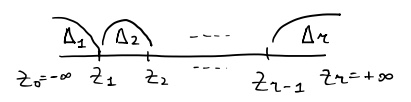
\includegraphics[scale=0.7]{comp1}
	\end{center}

	$m_i$: число $X_i$ в $\triangle_i$.\\
	$p_i^0 = P_0 (X_i \in \triangle_i) = F_0 (Z_i) - F_0 (Z_{i-1})$ (если верна $H_0$)\\
	$$\hat{\chi^2} = \underset{i=1}{\overset{r}{\sum}}\frac{(m_i - n p_i^0)^2}{n p_i^0} \xrightarrow[H_0]{d}\chi^2 (r-1)$$
\end{example}
\begin{example}[(критерий Фишера)]\label{lec:comp/example:2}
	$X = (X_1, \dots, X_n), \; H_0: F = F_0 (\theta_1, \dots, \theta_k)$.
	$$\hat{\chi^2} = \underset{i=1}{\overset{r}{\sum}}\frac{\left( m_i - n p_i^0 (\hat{\theta_1}, \dots, \hat{\theta_k}) \right)^2}{n p_i^0 (\hat{\theta_1}, \dots, \hat{\theta_k})} \xrightarrow[H_0]{d} \chi^2 (r-1-k)$$
\end{example}

\subsubsection*{Пример}\label{cha:compl/sec:nenorm/subsec:pirson/subsubsection:prob}

\textbf{Проверка на $N(0,1)$}

\begin{lstlisting}[language=Python]
	import numpy as np
	import pandas as pd
	import scipy.stats as stats
	
	def chisquare_normality_test(d, loc=None, scale=None, 
			min_bin_value=-3, max_bin_value=3, nbins=17):
	    :param d: array like -- initial data
	    :param loc: loc parameter of norm distribution
	    if loc is None then d.mean() is used
	    :param scale: scale parameter of norm distribution
	    if scale is None then d.std(ddof=0) is used
	    :param min_bin_value: right bound of the first bin
	    :param max_bin_value: left bound of the last bin
	    :param nbins: number of bins
    
	    bins = [-np.inf] + list(np.linspace(min_bin_value, max_bin_value, 
	    		max(nbins-1, 2))) + [np.inf]
	    
	    if loc is None and scale is None:
	        degrees_of_freedom = 2
	    elif loc is not None and scale is not None:
	        degrees_of_freedom = 0
	    else:
	        degrees_of_freedom = 1
	        
	    sf = np.histogram(d, bins)[0]
	    
	    loc = loc or d.mean()
	    scale = scale or d.std(ddof=0)

	    tf = [stats.norm.cdf(bins[i], loc=loc, scale=scale) - 
	    		
	    		stats.norm.cdf(bins[i-1], loc=loc, scale=scale) 
	                   for i in range(1, len(bins))]
	    tf = np.array(tf)*len(d)
	    
	    return stats.chisquare(sf, tf, ddof=degrees_of_freedom), 
	    		stats.chisquare(sf, tf, ddof=0)

	chisquare_normality_test(t_sample, nbins=27)
	chisquare_normality_test(norm_sample, loc=0, scale=2)
\end{lstlisting}

\section{Проверка на нормальность}\label{cha:compl/sec:norm}

\subsection{Тест Шапиро-Уилка}\label{cha:compl/sec:norm/subsec:shapiro}

\subsubsection*{Теория}\label{cha:compl/sec:norm/subsec:shapiro/subsubsection:theory}

Это наиболее мощный критерий проверки нормальности: $P(H_1|H_1) \to max$ среди всех. Работает корректно при $n < 5000$.
$$\begin{gathered}
	H_0: F \in \{N(a, \sigma^2)\}\\
	W = \frac{\left( \underset{i=1}{\overset{t}{\sum}}a_{n-i+1} (X_{(n-i+1)} - X_{(i)}) \right)^2}{\underset{i=1}{\overset{n}{\sum}}(X_i - \overline{X})^2}\\
	t = \begin{cases}
		\frac{n}{2}, \text{ если } n\% 2 =0 \\
		\frac{n-1}{2}, \text{ если } n\% 2 =1
	\end{cases}
\end{gathered}$$
При $H_0$ $W$ имеет табличное распределение, $C_{\text{кр}} = (-\infty, W_{\alpha})$.

\subsubsection*{Пример}\label{cha:compl/sec:nenorm/subsec:shapiro/subsubsection:prob}

\begin{lstlisting}[language=Python]
	stats.shapiro(norm_sample)
\end{lstlisting}

\subsection{Тест Харке-Бера}\label{cha:compl/sec:norm/subsec:ber}

\subsubsection*{Теория}\label{cha:compl/sec:norm/subsec:ber/subsubsection:theory}

$$\begin{gathered}
	H_0: F(x) \in \{N(a, \sigma^2)\} \\
	JB = \frac{n}{6} \left( (S_k)^2 + \frac{1}{4} (K_n)^2 \right) \\
	S_k = \frac{\hat{\mu_3}}{(\hat{\mu_2})^{\frac{3}{2}}}, \text{ Skewness - коэффициент ассиметрии} \\
	K_n = \frac{\hat{\mu_4}}{(\hat{\mu_2})^2}-3, \text{ Kurtosis - коэффициент эксцесса}\\
	\hat{\mu_j} = \frac{1}{n}\underset{i=1}{\overset{n}{\sum}}(X_i - \overline{X})^j
\end{gathered}$$
$$as = \frac{\mu_3}{(\mu_2)^{\frac{3}{2}}}, \text{ степень симметричности}$$
\begin{center}
	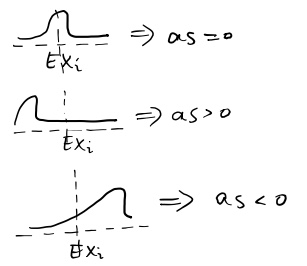
\includegraphics[scale=0.6]{comp2}
\end{center}
$$ex = \frac{\mu_4}{(\mu_2^2)}-3, \text{ степень остроконечности}$$
\begin{center}
	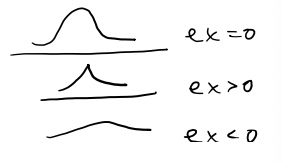
\includegraphics[scale=0.6]{comp3}
\end{center}

Тест работает корректно при $n > 2000$, тогда можно считать, что $JB \Hosim \chi^2 (2)$. Если $n < 2000$, то нужно смотреть таблицу квантилей.

\subsubsection*{Пример}\label{cha:compl/sec:nenorm/subsec:ber/subsubsection:prob}

\begin{lstlisting}[language=Python]
	stats.jarque_bera(norm_sample)
	res = stats.jarque_bera(norm_sample)
	statistics = res[0]
	p_value = 1 - stats.chi2.cdf(statistics, 2)
	p_value
\end{lstlisting}

\subsection{Тест Лиллиефорса}\label{cha:compl/sec:norm/subsec:lilli}

\subsubsection*{Теория}\label{cha:compl/sec:norm/subsec:lilli/subsubsection:theory}

До сих пор находится в разработке, периодически выдает ошибки (чаще всего на выборках объема больше 900). Если p-value получается больше 0.2, то выдает 0.2.\\
$H_0: F(x) = F_0 (x)$ - функция распределения $N(a, \sigma^2)$ - сложная гипотеза, параметры $a$ и $\sigma$ неизвестны. ($H_0: F \in \{N(a, \sigma^2)\}$)
$$\begin{gathered}
	T(x) = \sqrt{n} \; \underset{x}{sup} \; |\hat{F_n}(x) - F(x)| \\
	C_{\text{кр}} = [X_{1-\alpha}, +\infty), \; n > 30
\end{gathered}$$
$F(x)$ - функция распределения $N(\overline{X}, \hat{\sigma^2})$, $\overline{X}$ - ОМП, а для $\hat{\sigma^2}$ - $\frac{1}{n}\underset{i=1}{\overset{n}{\sum}}(X_i - X)^2$.\\
$F(x) = \Phi (\frac{X - \overline{X}}{\hat{\sigma}})$ - распределение Лиллиефорса.

\subsubsection*{Пример}\label{cha:compl/sec:nenorm/subsec:lilli/subsubsection:prob}

\begin{lstlisting}[language=Python]
	from statsmodels.stats.diagnostic import lilliefors
	short_t_sample = stats.t.rvs(4, size=800)
	lilliefors(short_t_sample)
\end{lstlisting}

\subsection{QQ Plot}\label{cha:compl/sec:norm/subsec:qq}

\subsubsection*{Теория}\label{cha:compl/sec:norm/subsec:qq/subsubsection:theory}

(Quantile Quantile Plot - вероятностная бумага)\\

\textbf{Проверка на $N(0,1)$}\\

$X = (X_1, \dots, X_n)$ из $N(0,1)$? $\Phi (x)$ - функция распределения $N(0,1)$. $\hat{F_n}(x) \approx \Phi(x)$. $\Phi^{-1} (\hat{F_n} (X_i)) \approx \Phi^{-1} (\Phi (X_i)) = X_i$. Рассмотрим точки $\left( \Phi^{-1} (\hat{F_n} (X_i)), \; \hat{F_n}^{-1}(\hat{F_n}(X_i)) \right)$, где первая координата - теоретический квантиль, а вторая - выборочный квантиль.
\begin{center}
	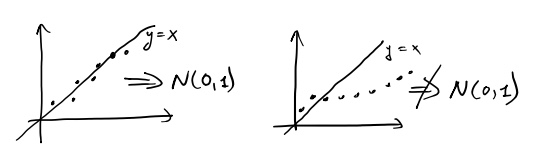
\includegraphics[scale=0.6]{comp4}
\end{center}

\textbf{Проверка на $N(a,\sigma^2)$}\\

$X = (X_1, \dots, X_n)$ из $N(a,\sigma^2)$? Вместо $y=x$ хотим увидеть $y = \sigma x + a$. $\hat{F_n}(x) \approx F_{N(a, \sigma^2)}(x)$. $\Phi^{-1} (\hat{F_N} (X)) \approx \Phi^{-1} (F_N (X)) = \Phi^{-1} (\Phi (\frac{X-a}{\sigma})) = \frac{X - a}{\sigma}$. Рассмотрим точки $\left( \frac{X_i - a}{\sigma}, X_i \right)$.
\begin{center}
	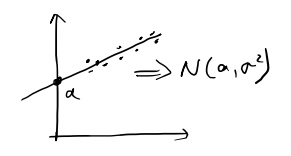
\includegraphics[scale=0.7]{comp5}
\end{center}

\subsubsection*{Пример}\label{cha:compl/sec:nenorm/subsec:qq/subsubsection:prob}

\begin{lstlisting}[language=Python]
	stats.probplot(norm_sample, plot=plt);
\end{lstlisting}

\subsection{Bootstrap}\label{cha:compl/sec:norm/subsec:bootstrap}

\subsubsection*{Теория}\label{cha:compl/sec:norm/subsec:bootstrap/subsubsection:theory}

Асимптотический ДИ:
$$\sqrt{n} \; (\hat{\theta_n} - \theta) \xrightarrow[]{d} N(0, \sigma^2(\theta)) \text{ -- АНО } \hat{\theta_n}$$
Проблемы:
\begin{itemize}
	\item[1)] $\sigma^2(\theta)$ сложно посчитать
	\item[2)] не знаем распределения выборки $X_i$
	\item[3)] $n$ не бесконечно большое
\end{itemize}
$X = (X_1, \dots, X_n)$ - выборка с неизветсной функцией распределения $F$.
$$T_n (X_1, \dots, X_n) \; \leftarrow \; \hat{\theta_n} (X_1, \dots, X_n) \text{ АНО}$$
Например, хотим оценить $D T_n$.\\

\textbf{Этап 1}\\
Рассмотрим реализацию $X_1, \dots, X_n$:
\begin{tabular}{| l | c | r |}
	\hline
	$X_1$ & $\dots$ & $X_n$ \\ \hline
	$\frac{1}{n}$ & $\dots$ & $\frac{1}{n}$ \\ \hline
\end{tabular} - дискретное распределение, это функция распределения $\hat{F_n}(x)$ (ЭФР).\\
Bootstrap -- создание одной или нескольких выборок $\hat{F_n}$ объема $n$. $\hat{F_n}(x) \approx F(x)$.\\

\textbf{Этап 2}\\
$D T_n$ -- ?\\
Сэмплируем $m$ бутстрэпных выборок: $\{ X_{i,1}^{*} \}_{i=1}^n, \dots,  \{X_{i,m}^{*} \}_{i=1}^n $. Вычисляем статистику на выборках: $T_{n,1}^{*}, \dots, T_{n,m}^{*}$. 
$$V_{boot} (T) = \hat{D T_n} = \frac{1}{m} \underset{j=1}{\overset{m}{\sum}}\left( T_{n,j}^{*} - \frac{1}{m}\underset{l=1}{\overset{m}{\sum}}T_{n,l}^{*} \right)^2, \;\; T^{*} = \frac{1}{m}\underset{l=1}{\overset{m}{\sum}}T_{n,l}^{*}$$

\textbf{Этап 3}\\
$T_n$ для АДИ:
$$\left( T_n - Z_{\frac{1+\gamma}{2}} \cdot \sqrt{V_{boot}(T)}, \; T_n + Z_{\frac{1+\gamma}{2}} \cdot \sqrt{V_{boot}(T)} \right)$$

\subsubsection*{Пример}\label{cha:compl/sec:nenorm/subsec:bootstrap/subsubsection:prob}

\begin{lstlisting}[language=Python]
	sample = pd.read_csv("Bootstrap_sample.txt")
	sample = sample['sample']
	n = len(sample)

	bootstrap = np.random.choice(sample, size=(100, n))
	v_boot = np.percentile(bootstrap, 50, axis=1).var()
	np.percentile(bootstrap, 50, axis=1)
	gamma=0.9
	g = (1 + gamma)/2.0
	(
    np.percentile(sample, 50) - stats.norm.ppf(g) * np.sqrt(v_boot),
    np.percentile(sample, 50) + stats.norm.ppf(g) * np.sqrt(v_boot)
	)
\end{lstlisting}
















\chapter{Корреляция}\label{cha:corr}

\section{Общие сведения}\label{cha:corr/sec:basic}

$$r = \frac{cov (\xi, \eta)}{\sqrt{D \xi} \sqrt{D \eta}} = \frac{E \xi \eta - E \xi E \eta}{\sqrt{D \xi} \sqrt{D \eta}} \in (-1,1)$$
\begin{itemize}
	\item[$\bullet$] $r = 1 \; \Rightarrow \; \xi = a \eta + b, \; a > 0$
	\item[$\bullet$] $r = -1 \; \Rightarrow \; \xi = a \eta + b, \; a < 0$
	\item[$\bullet$] $r = 0 \; \Rightarrow$ возможно $\xi$ и $\eta$ независимы, но не всегда: $\xi \sim N(0,1)$ и $\xi^2$ -- $corr (\xi, \xi^2) = 0$, но $\xi$ и $\xi^2$ не независимы. 
\end{itemize}
Т.о. корреляция - мера линейной зависимости.

\section{Выборочный коэффициент корреляции Пирсона}\label{cha:corr/sec:pirson}

\subsection*{Теория}\label{cha:corr/sec:pirson/subsec:theory}

Тест применяется для нормальных выборок, больших выборок без тяжелых хвостов. Тест не устойчив к выбросам. Строим точечную оценку корреляции. Хорошо ловит именно линейную зависимость.\\

$n$ объектов, $X$ и $Y$ - два признака.
$$\begin{gathered}
	r_{XY} = \frac{\frac{1}{n} \underset{}{\overset{}{\sum}}X_i Y_i - \overline{X} \overline{Y}}{\sigma_X \sigma_Y} \text{ - состоятельная оценка} \\
	\sigma_X = \sqrt{\frac{1}{n}\underset{i=1}{\overset{n}{\sum}}(X_i - \overline{X})^2}, \; \sigma_Y = \sqrt{\frac{1}{n}\underset{i=1}{\overset{n}{\sum}}(Y_i - \overline{Y})^2} \\
	r_{XY} = \frac{\sqrt{\underset{}{\overset{}{\sum}}(X_i - \overline{X})(Y_i - \overline{Y})}}{\sqrt{\underset{i=1}{\overset{n}{\sum}}(X_i - \overline{X})^2 \underset{i=1}{\overset{n}{\sum}}(Y_i - \overline{Y})^2}}
\end{gathered}$$
$H_0 : r = 0$.
$$T = \frac{r_{XY} \cdot \sqrt{n-2}}{\sqrt{1 - r_{XY}^2}} \Hosim t(n-2)$$

\subsection*{Пример}\label{cha:corr/sec:pirson/subsec:prob}

\begin{lstlisting}[language=Python]
	pearsonr(x, y)[0]
	pearsonr(x, y)[1]
	r = (np.mean(x*y) - np.mean(x)*np.mean(y))/(np.std(x) * np.std(y))
	from scipy.stats import t
	n=len(x)
	t_stat = (r * np.sqrt(n-2)) / np.sqrt(1 - r**2)
	p_value = 2*np.min([t.cdf(t_stat, n-2), 1 - t.cdf(t_stat, n-2)])
\end{lstlisting}

\section{Коэффициент корреляции Спирмана}\label{cha:corr/sec:spearman}

\subsection*{Теория}\label{cha:corr/sec:spearman/subsec:theory}

Тест непараметрический (применяется, если выборка ненормальна). Ловит монотонные распределения, более устойчив к выбросам.\\

Имеем $X = (X_1, \dots, X_n), \; Y = (Y_1, \dots, Y_n)$. $R_i$ - ранги $X_i$, $S_j$ - ранги $Y_j$. $\overline{R} = \overline{S} = \frac{n+1}{2}$.
$$\rho_S = \frac{\sqrt{\underset{}{\overset{}{\sum}}(R_i - \overline{R})(S_i - \overline{S})}}{\sqrt{\underset{i=1}{\overset{n}{\sum}}(R_i - \overline{R})^2 \underset{i=1}{\overset{n}{\sum}}(S_i - \overline{S})^2}}$$
$H_0:$ $X$ и $Y$ независимы, т.е. $E \rho_S = 0, \; D \rho_S = \frac{1}{n-1}$.\\

Асимптотический критерий для $n \ge 50$:
$$\frac{\rho_S}{\sqrt{D \rho_S}} = \sqrt{n-1} \; \rho_S \xrightarrow[H_0]{d}N(0,1)$$

\subsection*{Пример}\label{cha:corr/sec:spearman/subsec:prob}

\begin{lstlisting}[language=Python]
	spearmanr(x, y)[0]
	spearmanr(x, y)[1]
\end{lstlisting}

\section{Коэффициент корреляции Кендала}\label{cha:corr/sec:kendal}

\subsection*{Теория}\label{cha:corr/sec:kendal/subsec:theory}

\begin{definition}\label{lec:corr/def:1}
	$(X_i, Y_i)$ и $(X_j, Y_j)$ называются \blue{согласованными}, если $sgn (X_i - X_j) \cdot sgn (Y_i - Y_j) = 1$.
\end{definition}

$S$ - число согласованных пар, $R$ - число несогласованных пар. $T = S - R$. Всего пар $C_n^2 = \frac{n(n-1)}{2}, \; -\frac{n(n-1)}{2} \le T \le \frac{n(n-1)}{2}$.
$$\tau = \frac{2}{n(n-1)}T, \; -1 \le \tau \le 1$$
$H_0:$ $X$ и $Y$ независимы, т.е. $E \tau = 0, \; D \tau = \frac{2(2n+5)}{9n (n-1)}$.\\

Асимптотический критерий для $n \ge 50$:
$$\frac{\tau}{\sqrt{D \tau}} \xrightarrow[H_0]{d} N(0,1)$$
$H_1$ двусторонняя, свойства похожи на Спирмана.

\subsection*{Пример}\label{cha:corr/sec:kendal/subsec:prob}

\begin{lstlisting}[language=Python]
	kendalltau(x, y)[0]
	kendalltau(x, y)[1]
\end{lstlisting}

\section{Частная корреляция}\label{cha:corr/sec:chast}

\subsection*{Теория}\label{cha:corr/sec:chast/subsec:theory}

$$\rho_{XY|Z} = \frac{\rho_{XY} - \rho_{XZ} \cdot \rho_{YZ}}{\sqrt{(1-\rho_{XZ}^2)(1-\rho_{YZ})^2}}$$
$M \ge 3$ - общее число признаков $X_1, \dots, X_M$.\\
$\rho_{X_1 X_2 | X_3 \dots X_M} = -\frac{r_{12}}{r_{11} r_{22}}$, $\Sigma$ - матрица выборочных корреляций, $R = \Sigma^{-1}, \; R = (r_{ij})$.\\

$H_0:$ некоррелируемость $X_1$ и $X_2$ без $(X_3, \dots, X_M)$.
$$T = \frac{\rho \cdot \sqrt{n-M}}{\sqrt{1-\rho^2}} \Hosim t(n-M), \; \rho = \rho_{X_1 X_2 | X_3 \dots X_M}$$

\subsection*{Пример}\label{cha:corr/sec:chast/subsec:prob}

\begin{lstlisting}[language=Python]
	z = st.norm.rvs(size=1000, loc=0, scale=4) 
	x = z + st.norm.rvs(size=1000, loc=3, scale=1)
	y = z + st.norm.rvs(size=1000, loc=-2, scale=1)
	def partial_corr(x, y, z, method='pearson'):
    	if method == 'pearson':
       	 r_xy, r_xz, r_yz = pearsonr(x, y)[0], pearsonr(x, z)[0], 
       	 		pearsonr(y, z)[0]
    	elif method == 'kendall':
        	r_xy, r_xz, r_yz = kendalltau(x, y).correlation, 
        		kendalltau(x, z).correlation, kendalltau(y, z).correlation
   		else:
        	return None
    	return (r_xy - r_xz * r_yz) / np.sqrt((1 - r_xz ** 2) * 
    			(1 - r_yz ** 2))
    print ("pearson partial correlation:", 
    		partial_corr(x, y, z, method='pearson'))
\end{lstlisting}

\section{Таблицы сопряженности}\label{cha:corr/sec:contingency}

\subsection*{Теория}\label{cha:corr/sec:contingency/subsec:theory}

Пусть $A$ и $B$ - признаки, $A_1, \dots, A_r, B_1, \dots, B_s$ - значения. 

\begin{center}
	\begin{tabular}{| l || c | c | c | r |}
	\hline
	 & $B_1$ & $B_2$ & $\dots$ & $B_s$ \\ \hline \hline
	 $A_1$ & $\mu_{11}$ & $\mu_{12}$ & $\dots$ & $\mu_{1s}$ \\ \hline
	 $\vdots$ & $\vdots$ & $\vdots$ & $\ddots$ & $\vdots$ \\ \hline
	 $A_r$ & $\mu_{r1}$ & $\mu_{r2}$ & $\dots$ & $\mu_{rs}$ \\ \hline
	\end{tabular}
\end{center}

$H_0:$ $A$ и $B$ независимы.
$$\begin{gathered}
	\chi^2 = \underset{i=1}{\overset{r}{\sum}}\underset{j=1}{\overset{s}{\sum}}\frac{\left( \mu_{ij} - n \cdot \frac{\mu_{i \cdot}}{n} \cdot \frac{\mu_{\cdot j}}{n} \right)^2}{n \cdot \frac{\mu_{i \cdot}}{n} \cdot \frac{\mu_{\cdot j}}{n}} \xrightarrow[H_0]{d} \chi^2 \left( (r-1)(s-1) \right) \\
	\mu_{i \cdot} = \underset{j=1}{\overset{s}{\sum}}\mu_{ij}, \; \mu_{\cdot j} = \underset{i=1}{\overset{r}{\sum}}\mu_{ij} \\
	C_{\text{кр}} = [ \chi_{1-\alpha}^2 \left( (r-1)(s-1) \right), +\infty)
\end{gathered}$$

\hfill \break \hfill \break
Критерий Фишера:\\
$\tilde{r}$ - кол-во исходов
$$\hat{\chi^2} = \underset{i=1}{\overset{r}{\sum}}\frac{\left( m_i - n p_i (\hat{\theta_1}, \dots, \hat{\theta_k}) \right)^2}{n p_i (\hat{\theta_1}, \dots, \hat{\theta_k})} \xrightarrow[H_0]{d} \chi^2 (\tilde{r}-1-k) $$

\subsection*{Пример}\label{cha:corr/sec:contingency/subsec:prob}

\begin{problem}
	 Программные продукты оцениваются по шкале от 1 до 4 по качеству, и кроме того, имеется два способа написания программных продуктов: быстрый и медленный. Известно, что среди быстро написанных программных продуктов оценку 1 имеют 120 продуктов, оценку 2 – 124 продукта, 3 — 133 продукта, 4 – 106 продуктов. Среди медленно написанных продуктов оценку 1 имеют 97, 2 – 142, 3 – 129 и 4 – 149 продуктов. Выяснить, имеется ли статистически значимая связь между скоростью написания программных продуктов и их качеством (на уровне значимости 1$\%$ и на уровне значимости 3$\%$).
\end{problem}
\begin{solution}
	\begin{lstlisting}[language=Python]
		table = np.array([[120, 124, 133, 106],
		[97, 142, 129, 149]])

		st.chi2_contingency(table)
		st.chi2_contingency(table)[1]
	\end{lstlisting}
\end{solution}

\begin{problem}
	 Проверка независимости двух признаков с помощью таблиц сопряженности
\end{problem}
\begin{solution}
	\begin{lstlisting}[language=Python]
		Star = pd.read_csv("Star.csv")
		x = Star['x']
		y = Star['y']
		Star['x_bin'] = pd.cut(x, [-np.inf, -0.5, 0.5, np.inf])
		Star['y_bin'] = pd.cut(y, [-np.inf, -0.5, 0.5, np.inf])

		table2 = Star.pivot_table(values='x', index='x_bin', columns='y_bin', aggfunc='count', fill_value=0)

		res = st.chi2_contingency(table2)
		p_value = res[1]
	\end{lstlisting}
\end{solution}




















\chapter{Сравнение двух выборок}\label{cha:2sample}

\section{Сравнение средних (медиан)}\label{cha:2sample/sec:mo}

\subsection{Парные (зависимые выборки)}\label{cha:2sample/sec:mo/subsec:pair}

Признаки:
\begin{itemize}
	\item[$\bullet$] одинаковый размер выборок
	\item[$\bullet$] строгое соответствие $X_i \leftrightarrow Y_i$
\end{itemize}
Примеры:
\begin{itemize}
	\item[$\bullet$] <<до и после>>
	\item[$\bullet$] один и тот же показатель двумя способами
\end{itemize}

Сводим к одной выборке: $Z_i = Y_i - X_i$.

	\subsubsection{t-test 2 sample}\label{cha:2sample/sec:mo/subsec:pair/subsubsec:ttest}

		\paragraph*{Теория}\label{cha:2sample/sec:mo/subsec:pair/subsubsec:ttest/par:theory}

		Применяем, если $X$ и $Y$ - две нормальные выборки.\\

		$$\begin{gathered}
			Z_i = Y_i - X_i \\
			H_0: E Z_i = 0 \; \Leftrightarrow \; H_0: E X_i = E Y_i\\
		\end{gathered}$$

		Применяем t-test:
		$$t = \frac{\overline{Z}}{\frac{S_Z}{\sqrt{n}}} \Hosim t(n-1)$$

		\paragraph*{Пример}\label{cha:2sample/sec:mo/subsec:pair/subsubsec:ttest/par:prob}

		\begin{problem}
			Было проведено исследование, чтобы выяснить, повлияют ли новые диетические медикаменты на женщин, желающих сбросить вес. Вес 100 пациенток был измерен до лечения и через 6 недель ежедневного применения лечения. Данные приведены в файле "Weight.txt". При уровне значимости 5$\%$ можно ли сделать вывод, что лечение уменьшает вес?
		\end{problem}
		\begin{solution}
			\begin{lstlisting}[language=Python]
				data = pd.read_csv("Weight.txt")
				x = data['x']
				y = data['y']
				st.shapiro(x)
				st.shapiro(y)
				from scipy.stats import ttest_rel
				ttest_rel(x, y)
				t_test_res = ttest_rel(x, y)
				t_test_res.pvalue/2.0
			\end{lstlisting}
			Вручную:
			\begin{lstlisting}[language=Python]
				z = y - x
				from scipy.stats import t
				n = len(z)
				z_mean = np.mean(z)
				z_s = np.std(z, ddof=1)
				t_stat = (z_mean - 0) * np.sqrt(n) / z_s
				t_p_value = t.cdf(t_stat, n-1)
				t_p_value
			\end{lstlisting}
		\end{solution}

	\subsubsection{Критерий знаков}\label{cha:2sample/sec:mo/subsec:pair/subsubsec:signes}

		\paragraph*{Теория}\label{cha:2sample/sec:mo/subsec:pair/subsubsec:signes/par:theory}

		Является непараметрическим критерием, применяется, когда выборки не нормальны.\\

		$Z_i = Y_i - X_i$, $Z_i = \theta + e_i$, где $\theta$ - эффект обработки, $e_i$ - взаимно независимые случайные величины из непрерывной совокупности такой, что $P (e_i < 0) = P(e_i > 0) = \frac{1}{2}$.\\

		$H_0: \theta = 0$. $\psi_i = \begin{cases}
			1, \; Z_i > 0 \\
			0, \; Z_i < 0
		\end{cases}$. Отбрасываем $Z_i = 0$ и уменьшаем $n$. $B = \underset{i=1}{\overset{n}{\sum}}\psi_i$ - число пар таких, что $Y_i > X_i$. $B \Hosim Bin (n, \frac{1}{2})$.\\

		Асимптотический критерий: $B^{*} = \frac{B - \frac{n}{2}}{\sqrt{\frac{n}{4}}} \xrightarrow[H_0]{d}N(0,1)$.

		\paragraph*{Пример}\label{cha:2sample/sec:mo/subsec:pair/subsubsec:signes/par:prob}

		\begin{lstlisting}[language=Python]
			z = z[z!=0] 
			b = sum(z > 0)
			n = len(z)

			from scipy.stats import binom_test
			binom_test(b, n,  p=0.5)

			sign_res=binom_test(b, n,  p=0.5)
			sign_res/2.0

			from scipy.stats import binom
			binom.cdf(b, n, 0.5)

			b_star = (b - n*0.5) / np.sqrt(n*0.25)
			from scipy.stats import norm
			norm.cdf(b_star, loc=0, scale=1)
		\end{lstlisting}

	\subsubsection{Знакоранговый критерий Вилкоксона}\label{cha:2sample/sec:mo/subsec:pair/subsubsec:wilcox}

		\paragraph*{Теория}\label{cha:2sample/sec:mo/subsec:pair/subsubsec:wilcox/par:theory}

		Является непараметрическим критерием, применяется, когда выборки не нормальны. Применяется при $n > 20$.\\

		$Z_i = Y_i - X_i$, $Z_i = \theta + e_i$, где $\theta$ - эффект обработки, $e_i$ - взаимно независимые случайные величины из непрерывной совокупности и симметричные относительно 0.\\

		$H_0: \theta = 0$. Сортируем $|Z_1|, \dots, |Z_n|$ по возрастанию. $R_i$ - ранг $Z_i$. $\psi_i = \begin{cases}
			1, \; Z_i > 0 \\
			0, \; Z_i < 0
		\end{cases}$. Отбрасываем $Z_i = 0$ и уменьшаем $n$. $T^{+} = \underset{i=1}{\overset{n}{\sum}}R_i \psi_i$.\\

		Асимптотический критерий: $\frac{T^{*} - \frac{n(n+1)}{4}}{\sqrt{\frac{n(n+1)(2n+1)}{24}}} \xrightarrow[H_0]{d} N(0,1)$.

		\paragraph*{Пример}\label{cha:2sample/sec:mo/subsec:pair/subsubsec:wilcox/par:prob}

		\begin{lstlisting}[language=Python]
			from scipy.stats import wilcoxon
			wilcoxon(x, y)
			signed_rank_res = wilcoxon(x, y)
			signed_rank_res.pvalue/2.0
		\end{lstlisting}

\subsection{Независимые выборки}\label{cha:2sample/sec:mo/subsec:nes}

Признаки:
\begin{itemize}
	\item[$\bullet$] может быть разный размер выборок
	\item[$\bullet$] выборки взяты <<из разных мест>> независимо друг от друга
\end{itemize}
Примеры:
\begin{itemize}
	\item[$\bullet$] врачи из разных городов
\end{itemize}

	\subsubsection{F-test 2 sample}\label{cha:2sample/sec:mo/subsec:pair/subsubsec:ftest}

	Применяется, если выборки нормальны. Используем F-test для установления равенства или неравенства дисперсий.

		\paragraph{t-test 2 sample}\label{cha:2sample/sec:mo/subsec:pair/subsubsec:ftest/par:ttest}

			\subparagraph*{Теория}\label{cha:2sample/sec:mo/subsec:pair/subsubsec:ftest/par:ttest/subpar:theory}

			Применяется, если имеем неизвестные равные дисперсии.

			$X_i \sim N(a_1, \sigma_1^2), \; Y_i \sim N(a_2, \sigma_2^2)$. После F-testа устанавливаем, что $\sigma_1^2 = \sigma_2^2$. $H_0: E X_i = E Y_j$.
			$$\begin{gathered}
				t = \frac{\overline{X} - \overline{Y}}{\sqrt{S_p^2 (\frac{1}{n} + \frac{1}{m})}} \Hosim t(n+m-2) \\
				S_p^2 = \frac{(n-1)S_x^2 + (m-1)S_y^2}{n+m-2} \text{ (pooled variance estimator)}
			\end{gathered}$$

			\subparagraph*{Пример}\label{cha:2sample/sec:mo/subsec:pair/subsubsec:ftest/par:ttest/subpar:prob}

			\begin{problem}
				Для сравнения уровня заработной платы были отобраны в соответствии со стажем работники-мужчины и работники-женщины. В файлах "Male.txt" и "Female.txt" содержатся получившиеся данные (в тысячах рублей). Можно ли утверждать на уровне значимости 5$\%$, что зарплата женщин ниже?
			\end{problem}
			\begin{solution}
				\begin{lstlisting}[language=Python]
					data1 = pd.read_csv("Male.txt")
					male = data1['male']
					data2 = pd.read_csv("Female.txt")
					female = data2['female']
					st.shapiro(male)
					st.shapiro(female)

					from scipy.stats import f
					def F_test(x, y):
					    x = np.array(x)
					    y = np.array(y)
					    df1 = len(x) - 1
					    df2 = len(y) - 1
					    F_stat = np.var(x, ddof=1)/np.var(y, ddof=1)
					    pv = 2*np.min([f.cdf(F_stat, df1, df2), 1 - f.cdf(F_stat, df1, df2)])
					    return pv
					
					F_test(male, female)

					from scipy.stats import ttest_ind
					ttest_ind(male, female, equal_var=False)
					t_res = ttest_ind(male, female, equal_var=False)
					t_res.pvalue/2.0
				\end{lstlisting}
			\end{solution}

		\paragraph{Критерий Аспина-Уэлса}\label{cha:2sample/sec:mo/subsec:pair/subsubsec:ftest/par:wales}

			\subparagraph*{Теория}\label{cha:2sample/sec:mo/subsec:pair/subsubsec:ftest/par:wales/subpar:theory}

			Применяется, если имеем неизвестные разные дисперсии.

			$X_i \sim N(a_1, \sigma_1^2), \; Y_i \sim N(a_2, \sigma_2^2)$. После F-testа устанавливаем, что $\sigma_1^2 \not = \sigma_2^2$. $H_0: E X_i = E Y_j$.
			$$\begin{gathered}
				t = \frac{\overline{X} - \overline{Y}}{\sqrt{\frac{S_x^2}{n} + \frac{S_y^2}{m}}} \Hosim t(d.f.) \\
				d.f. = \frac{\left( \frac{S_x^2}{n} + \frac{S_y^2}{m} \right)^2}{\frac{\left( \frac{S_x^2}{n} \right)^2}{n-1} + \frac{\left( \frac{S_y^2}{m} \right)^2}{m-1}} \text{ (берем ближайшее целое число)}
			\end{gathered}$$

			При больших $n$ и $m$ статистика $t \Hosim N(0,1)$.

			\subparagraph*{Пример}\label{cha:2sample/sec:mo/subsec:pair/subsubsec:ftest/par:wales/subpar:prob}

			надо реализовать

	\subsubsection{Критерий ранговых сумм Вилкоксона}\label{cha:2sample/sec:mo/subsec:pair/subsubsec:wilcox}

		\paragraph*{Теория}\label{cha:2sample/sec:mo/subsec:pair/subsubsec:wilcox/par:theory}

		Является непараметрическим тестом, применятся в случае ненормальности выборок.

		$X_i = e_i, i = \ton n$, $Y_j = e_{n+j} + \triangle$, где $\triangle$ - сдвиг. $e_1, \dots, e_n$ - значения $X$, $e_{n+1}, \dots, e_{n+m}$ - значения $Y$. Значения взаимно независимы и из одной непрерывной совокупности.

		$H_0: \triangle = 0$ (нет повторов). Рассмотрим $N = n+m$ наблюдений. От $min$ к $max$ $R_j$ -- ранг $Y_j$. Статистика: $W = \underset{j=1}{\overset{m}{\sum}}R_j$.\\

		\textit{Замечание}: рассматриваем ранги $X_i$, тогда:
		$$W' = \frac{(n+m)(n+m+1)}{2}-W$$
		Асимптотический критерий при $n,m > 20$:
		$$\frac{W - \frac{m (n+m+1)}{2}}{\sqrt{\frac{n m (n+m+1)}{12}}} \xrightarrow[H_0]{d} N(0,1)$$

		\paragraph*{Пример}\label{cha:2sample/sec:mo/subsec:pair/subsubsec:wilcox/par:prob}

		надо реализовать

	\subsubsection{Критерий Манна и Уитни}\label{cha:2sample/sec:mo/subsec:pair/subsubsec:mann}

		\paragraph*{Теория}\label{cha:2sample/sec:mo/subsec:pair/subsubsec:mann/par:theory}

		Является непараметрическим тестом, применятся в случае ненормальности выборок.

		$H_0: \triangle = 0$. Вместо $W$ рассмотрим:
		$$\begin{gathered}
			U = \underset{i=1}{\overset{n}{\sum}}\underset{j=1}{\overset{m}{\sum}}\mathbb{I}(X_i < Y_j) \\
			W = U + \frac{m(m+1)}{2}
		\end{gathered}$$
		Асимптотический критерий:
		$$\frac{U - \frac{n m }{2}}{\sqrt{\frac{n m (n+m+1)}{12}}} \xrightarrow[H_0]{d} N(0,1)$$

		\paragraph*{Пример}\label{cha:2sample/sec:mo/subsec:pair/subsubsec:mann/par:prob}

		\begin{lstlisting}[language=Python]
			from scipy.stats import mannwhitneyu
			mannwhitneyu(female, male, alternative='less')
			res = mannwhitneyu(female, male, alternative='less')
			res.pvalue
		\end{lstlisting}

\section{Сравнение дисперсий}\label{cha:2sample/sec:var}

Пусть $X = (X_1, \dots, X_n)$ и $Y = (Y_1, \dots, Y_n)$ -- две независимые выборки. $H_0: D X_i = D Y_j$. $H_1: D X_i \not = D Y_j$. 

\subsection{F-test 2 sample}\label{cha:2sample/sec:var/subsec:ftest}

	\subsubsection*{Теория}\label{cha:2sample/sec:var/subsec:ftest/subsubsec:theory}

	Применяется, если обе выборки нормальные.\\

	$X_i \sim N(a_1, \sigma_1^2), \; Y_j \sim N(a_2, \sigma_2^2)$ - независимые выборки. $H_0: \sigma_1^2 = \sigma_2^2$. $H_1: \sigma_1^2 \not = \sigma_2^2$.
	$$F = \frac{S_X^2}{S_Y^2} \Hosim F (n-1, m-1)$$

	\subsubsection*{Пример}\label{cha:2sample/sec:var/subsec:ftest/subsubsec:prob}

	надо реализовать

\subsection{Критерий Зигеля-Тьюки}\label{cha:2sample/sec:var/subsec:siegel}

	\subsubsection*{Теория}\label{cha:2sample/sec:var/subsec:siegel/subsubsec:theory}

	Рассмотрим $N = n+m$. Сортируем от $min$ к $max$, где $Z$ - объединенные $X$ и $Y$: $Z_{(1)} \le Z_{(2)} \le \dots \le Z_{(n-1)} \le Z_{(n)}$. Присваиваем ранги двигаясь от краев к центру последовательности, чередуя начало и конец последовательности, т.е.: ранг 1 имеет $Z_{(1)}$, ранг 2 -- $Z_{(n)}$, ранг 3 -- $Z_{(2)}$ и т.д.\\
	$T = \underset{i=1}{\overset{n}{\sum}}\tilde{rank} (X_i)$.\\

	Асимптотический критерий:
	$$\frac{T - \frac{n (n+m+1)}{2}}{\sqrt{\frac{n m (n+m+1)}{2}}} \xrightarrow[H_0]{d} N(0,1)$$

	\subsubsection*{Пример}\label{cha:2sample/sec:var/subsec:siegel/subsubsec:prob}

	надо реализовать




























\chapter{Проверка на однородность}\label{cha:uniform}

Используется только для непрерывных распределений.\\

\section{Сравнение двух выборок}\label{cha:uniform/sec:2}

Пусть $X = (X_1, \dots, X_n)$ имеет распределение $F$, $Y = (Y_1, \dots, Y_n)$ имеет распределение $G$. $X$ и $Y$ - две независимые выборки.\\
$H_0: F = G$.

	\subsection{Критерий Смирного}\label{cha:uniform/sec:2/smirn}

		\subsubsection*{Теория}\label{cha:uniform/sec:2/subsec:smirn/subsubsec:theory}

		Является непараметрическим критерием.

		$$T = \sqrt{\frac{n m }{n+m}}\cdot \underset{x \in \mathbb{R}}{sup} \; |\hat{F_n}(x) - \hat{G_m}(x)|$$
		Асимптотический критерий:
		$$\begin{gathered}
			T \xrightarrow[H_0]{d}\xi, \;\; \xi \text{ имеет распределение Колмогорова} \\
			C_{\text{кр}} = [K_{1-\alpha}, +\infty)
		\end{gathered}$$

		\subsubsection*{Пример}\label{cha:uniform/sec:2/subsec:smirn/subsubsec:prob}

		\begin{lstlisting}[language=Python]
			from scipy.stats import norm, t
			x = norm.rvs(size = 200, loc = 0, scale = 1)
			y = t.rvs(size=300, df = 7)
			z = norm.rvs(size = 400, loc = 0, scale = 3)
			from scipy.stats import ks_2samp
			s_2samp(x, y)
			ks_2samp(x, z)
		\end{lstlisting}

\section{Сравнение $k \ge 2$ выборок}\label{cha:uniform/sec:k}

	\subsection{Общий критерий Андерсона-Дарлинга}\label{cha:uniform/sec:k/andersdarling}

		\subsubsection*{Теория}\label{cha:uniform/sec:k/subsec:andersdarling/subsubsec:theory}

		Является непараметрическим критерием.\\

		Имеем $k \ge 2$ независимых выборок. $(X_{11}, \dots, X_{1 n_1})$ имеет распределение $F_1$, $\dots$, $(X_{k1}, \dots, X_{k n_k})$ имеет распределение $F_k$. $H_0: F_1 = \dots = F_k$. $\hat{F_1}, \dots, \hat{F_k}$ - ЭФР, $N = n_1 + \dots + n_k$. $\hat{H_N}(x)$ -- ЭФР по всей совокупности из $N$ наблюдений.
		$$\Omega^2 = \underset{i=1}{\overset{k}{\sum}}n_i \cdot \underset{\mathbb{R}}{\overset{}{\int}}\frac{\left( \hat{F_i}(x) - \hat{H_N}(x) \right)^2}{\hat{H_N}(x) (1 - \hat{H_N}(x))} d \hat{H_N}(x)$$ 

		\subsubsection*{Пример}\label{cha:uniform/sec:k/subsec:andersdarling/subsubsec:prob}

		В качестве результата тест выдает значение статистики, набор квантилей $x_{1-\alpha}$ для значений $\alpha$ вида 25$\%$, 10$\%$, 5$\%$, 2.5$\%$, 1$\%$, 0.5$\%$, 0.1$\%$ и p-value.

		\begin{lstlisting}[language=Python]
			from scipy.stats import anderson_ksamp
			anderson_ksamp([x, y])
		\end{lstlisting}

	\subsection{Критерий Краскела-Уоллиса}\label{cha:uniform/sec:k/kraskel}

		\subsubsection*{Теория}\label{cha:uniform/sec:k/subsec:kraskel/subsubsec:theory}

		Применяется в непараметрическом случае (хотя бы одна выборка ненормальна).\\

		Имеем $k \ge 2$ выборок:
		$$\begin{pmatrix}
			X_{11} \\ \vdots \\ X_{n_1 1}
		\end{pmatrix}, \begin{pmatrix}
			X_{12} \\ \vdots \\ X_{n_2 2}
		\end{pmatrix}, \dots, \begin{pmatrix}
			X_{1k} \\ \vdots \\ X_{n_k k}
		\end{pmatrix}$$

		Для элемента $X_{ij}$ $i$ - это номер элемента в $j$-ой выборке, а $j$ - это номер выборки. $N = \underset{j=1}{\overset{k}{\sum}}n_j$.\\

		$X_{ij} = \mu + \beta_j + \varepsilon_{ij}$, где $\beta_j$ - эффект от воздействия фактора, $\varepsilon_{ij}$ - случайные ошибки. Необходимо, чтобы были выполнены следующие условия:
		\begin{itemize}
			\item[$\bullet$] все $\varepsilon_{ij}$ независимы
			\item[$\bullet$] все $\varepsilon_{ij}$ имеют одинаковое непрерывное распределение
		\end{itemize}
		$H_0: \beta_1 = \dots = \beta_k$. $H_1:$ не все $\beta_j$ равны. Строим статистику: смешиваем все $N$ наблюдений, $R_{ij}$ - ранг $X_{ij}$, $S_j = \underset{i=1}{\overset{n_j}{\sum}}R_{ij}$ - сумма рангов $j$-ой выборки, $R_{\cdot j} = \frac{S_j}{n_j}$ - средний ранг $j$-ой выборки, $R_{\cdot \cdot} = \frac{1}{N}\underset{i,j}{\overset{}{\sum}}R_{ij} = \frac{N+1}{2}$ - общий средний ранг.
		$$\begin{gathered}
			H = \frac{12}{N(N+1)}\cdot \underset{j=1}{\overset{k}{\sum}}n_j (R_{\cdot j} - R_{\cdot \cdot})^2 = \left[ \frac{12}{N (N+1)} \cdot \underset{j=1}{\overset{k}{\sum}}\frac{S_j^2}{n_j} \right] - 3 (N+1) \\
			H \xrightarrow[H_0]{} \text{ табличное распределение}\\
			C_{\text{кр}} = [h_{1-\alpha}, +\infty)
		\end{gathered}$$
		Асимптотический критерий:
		$$H \xrightarrow[H_0]{d}\chi^2 (k-1), \; \; C_{\text{кр}} = [ \chi_{1-\alpha}^2 (k-1), +\infty)$$

		\subsubsection*{Пример}\label{cha:uniform/sec:k/subsec:kraskel/subsubsec:prob}

		\begin{problem}
			В файле «Harvest.txt» представлены данные об урожае клубники (в квартах) с участков трех типов почв. Влияет ли (на уровне значимости 5$\%$) тип почвы на урожайность?
		\end{problem}
		\begin{solution}
			\begin{lstlisting}[language=Python]
				data = pd.read_csv("Harvest.txt")
				x = data['x']
				y = data['y']
				z = data['z']
				st.shapiro(x)
				st.shapiro(y)
				st.shapiro(z)
				from scipy.stats import kruskal
				kruskal (x, y, z)
			\end{lstlisting}
		\end{solution}

	\subsection{Критерий Джонкхиера}\label{cha:uniform/sec:k/john}

		\subsubsection*{Теория}\label{cha:uniform/sec:k/subsec:john/subsubsec:theory}

		$H_0: \beta_1 = \dots = \beta_k$, $H_1: \beta_1 \le \beta_2 \le \dots \le \beta_k$ - альтернатива возрастания влияния фактора. Данный тест имеет большую мощность при такой альтернативе, чем тест Краскела-Уоллеса.\\

		Статистика: $C_k^2 = \frac{k(k-1)}{2}$ - кол-во пар выборок. Считает $\frac{k(k-1)}{2}$ значений статистики Манна-Уитни.
		$$\begin{gathered}
			U_{rs} = \underset{i=1}{\overset{n_r}{\sum}}\underset{j=1}{\overset{n_s}{\sum}}\mathbb{I}(X_{i r} < X_{j s}), \;\; 1 \le r \le s \le k \\
			J = \underset{r < s}{\overset{}{\sum}}U_{rs} = \underset{r=1}{\overset{k-1}{\sum}}\underset{s=r+1}{\overset{k}{\sum}}U_{rs} \text{ -- имеет табличное распределение}\\
			C_{\text{кр}} = [j_{1-\alpha}, +\infty)
		\end{gathered}$$
		Асимптотический критерий:
		$$\begin{gathered}
			J^{*} = \frac{J - E J}{\sqrt{D J}} \xrightarrow[H_0]{d}N(0,1) \\
			H_0 \; \Rightarrow \; \begin{cases}
				E J = \frac{1}{4}\left( N^2 - \underset{j=1}{\overset{k}{\sum}}n_j^2 \right) \\
				D J = \frac{1}{72} \left( N^2 (2N +3) - \underset{j=1}{\overset{k}{\sum}}n_j^2 (2n_j + 3) \right)
			\end{cases}
		\end{gathered}$$

		\subsubsection*{Пример}\label{cha:uniform/sec:k/subsec:john/subsubsec:prob}

		надо реализовать

	\subsection{Критерий Неменьи}\label{cha:uniform/sec:k/nemeni}

		\subsubsection*{Теория}\label{cha:uniform/sec:k/subsec:nemeni/subsubsec:theory}

		Nemenyi test принадлежит семейству Post Hoc tests - они мощнее, чем попарный t-test, а также легки в подсчете.\\

		$H_0: \beta_r = \beta_s$, $H_1: \beta_r \not = \beta_s$.
		$$\begin{gathered}
			T = \frac{R_{\cdot r} - R_{\cdot s}}{\sqrt{\frac{N(N+1)}{24}\left( \frac{1}{n_r} + \frac{1}{n_s} \right)}} \sim \text{ табличное распределение} \\
			|T| > q_{\text{crit}} \; \Rightarrow \; \text{отвергаем } H_0
		\end{gathered}$$

		Желательно делать поправку на множественное сравнение.

		\subsubsection*{Пример}\label{cha:uniform/sec:k/subsec:nemeni/subsubsec:prob}

		\begin{lstlisting}[language=Python]
			import scikit_posthocs as sp
			sp.posthoc_nemenyi([x, y, z])
			nem_res = sp.posthoc_nemenyi([x, y, z])
			nem_res[1][2]
		\end{lstlisting}

	\subsection{Критерий Бартлетта}\label{cha:uniform/sec:k/bartlet}

		\subsubsection*{Теория}\label{cha:uniform/sec:k/subsec:bartlet/subsubsec:theory}

		Применяется в предположении, что $X_{ij}\sim N (\mu_j, \sigma_j^2)$, параметры распределения неизвестны. Критерий применяется для получения информации про дисперсию.\\

		$H_0: \sigma_1 = \dots = \sigma_k$, $H_1:$ не все $\sigma_j$ равны. Статистика:
		$$\begin{gathered}
			B^{*} = \gamma^{-1} \cdot N \cdot \ln B, \text{ где}\\
			\;\;\;\; \gamma = 1 + \frac{1}{3(k-1)} \left[ \underset{j=1}{\overset{k}{\sum}}\frac{1}{n_j} - \frac{1}{N} \right] \\
			B = \frac{\left( \frac{1}{N} \underset{j=1}{\overset{k}{\sum}}n_j S_j^2 \right)}{\sqrt[N]{\underset{j=1}{\overset{k}{\Pi}} (S_j^2)^{n_j}}} \\
			S_j^2 = \frac{1}{n_j - 1} \underset{i=1}{\overset{n_j}{\sum}}(X_{ij} - X_{\cdot j})^2
		\end{gathered}$$
		При $n_j \ge 3$ $B^{*} \Hosim \chi^2 (k-1)$.\\

		При отвержении $H_0$ возникает проблема множественных сравнений, поэтому необходимо делать \blue{поправку Бонферонни}: $\alpha \to \frac{\alpha}{C_k^2} = \tilde{\alpha}$.

		\subsubsection*{Пример}\label{cha:uniform/sec:k/subsec:bartlet/subsubsec:prob}

		\begin{lstlisting}[language=Python]
			from scipy.stats import bartlett
			bartlett(x, y, z)
		\end{lstlisting}

	\subsection{Критерий Данна}\label{cha:uniform/sec:k/dann}

		\subsubsection*{Теория}\label{cha:uniform/sec:k/subsec:dann/subsubsec:theory}

		Является непараметрическим тестом, применяется для больших выборок, т.е. является асимптотическим.\\

		$H_0: \beta_r = \beta_s$, $H_1: \beta_r \not = \beta_s$.
		$$T = \frac{R_{\cdot r} - R_{\cdot s}}{\sqrt{\frac{N(N+1)}{12}\left( \frac{1}{n_r} + \frac{1}{n_s} \right)}}$$

		\begin{center}
			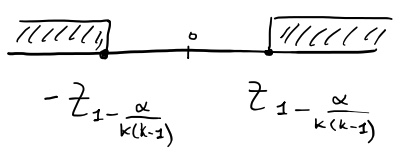
\includegraphics[scale=0.6]{uniform1}
		\end{center}

		$$1 - \frac{\alpha}{2} \to 1 - \frac{\alpha}{C_k^2 \cdot 2} = 1 - \frac{\alpha}{k (k-1)}$$

		\subsubsection*{Пример}\label{cha:uniform/sec:k/subsec:dann/subsubsec:prob}

		\begin{lstlisting}[language=Python]
			sp.posthoc_dunn([x, y, z], p_adjust = 'bonferroni')
			dunn_res = sp.posthoc_dunn([x, y, z], p_adjust = 'bonferroni')
			dunn_res[1][3]
			dunn_res = sp.posthoc_dunn([x, y, z], p_adjust = None)
			dunn_res[1][3]*3
		\end{lstlisting}

	\subsection{ANOVA}\label{cha:uniform/sec:k/anova}

		\subsubsection*{Теория}\label{cha:uniform/sec:k/subsec:anova/subsubsec:theory}

		Применяется в случае $k$ нормальных выборок - однофакторный дисперсионный анализ: ANOVA = Analysis of Variance. \\

		$X_{ij} \sim N(\mu_j, \sigma^2)$. Для применения необходимо выполнния следующих условий:
		\begin{itemize}
			\item[$\bullet$] нормальное распределение всех выборок
			\item[$\bullet$] равенство дисперсий всех выборок
			\item[$\bullet$] независимость наблюдений
		\end{itemize}

		$H_0: \mu_1 = \dots = \mu_k$, $H_1:$ не все $\mu_j$ равны. Строим статистику:
		$$\begin{gathered}
			X_{\cdot j} = \frac{1}{n_j}\underset{i=1}{\overset{n_j}{\sum}}X_{ij} = \overline{X_j} \text{ - среднее } j\text{-ой выборки}\\
			X_{\cdot \cdot} = \frac{1}{N} \underset{j=1}{\overset{k}{\sum}}\underset{i=1}{\overset{n_j}{\sum}}X_{ij}\\
			F = \frac{N-k}{k-1}\cdot \frac{\underset{j=1}{\overset{k}{\sum}}n_j (X_{\cdot j} - X_{\cdot \cdot})^2}{\underset{j=1}{\overset{k}{\sum}}\underset{i=1}{\overset{n_j}{\sum}}(X_{ij} - X_{\cdot j})^2} \Hosim F(k-1, N-k)
		\end{gathered}$$

		Если $n_1 = \dots = n_k$, то при небольшом отклонении от нормальности распределений и от равенства дисперсий ANOVA все равно можно применять.

		\subsubsection*{Пример}\label{cha:uniform/sec:k/subsec:anova/subsubsec:prob}

		\begin{lstlisting}[language=Python]
			from scipy.stats import f_oneway
			f_oneway(x, y, z)
		\end{lstlisting}

	\subsection{LSD Фишера}\label{cha:uniform/sec:k/lsd}

		\subsubsection*{Теория}\label{cha:uniform/sec:k/subsec:lsd/subsubsec:theory}

		Fisher's least significant difference test применяется в предположении нормальности данных. $X_{ij} \sim N(\mu_j, \sigma^2)$. Дисперсии равны, выборки независимы.\\

		$H_0: \mu_r = \mu_s$, $H_1: \mu_r \not = \mu_s$.
		$$\begin{gathered}
			T = \frac{X_{\cdot r} - X_{\cdot s}}{\sqrt{MS_E \left( \frac{1}{n_r} + \frac{1}{n_s} \right)}} \Hosim t (N-k), \text{ где}\\
			X_{\cdot r} = \frac{1}{n_r} \underset{i=1}{\overset{n_r}{\sum}}X_{ir}, \; MS_E = \frac{SS_E}{N_k}, \; SS_E = \underset{j=1}{\overset{k}{\sum}}\underset{i=1}{\overset{n_j}{\sum}}(X_{ij} - X_{\cdot j})^2 = \underset{j=1}{\overset{k}{\sum}}(n_j - 1)S_j^2
		\end{gathered}$$

		\subsubsection*{Пример}\label{cha:uniform/sec:k/subsec:lsd/subsubsec:prob}

		\begin{lstlisting}[language=Python]
			def LSD_Fisher(i, j, samples):
			    n1, n2 = len(samples[i]), len(samples[j])
			    k = len(samples)
			    N = np.sum([len(samples[l]) for l in range(k)])
			    SSe = np.sum([np.var(samples[l], ddof=0) * len(samples[l]) for l in range(k)])
			    stat = (np.mean(samples[i]) - np.mean(samples[j]))/np.sqrt(SSe / (N - k) * (1.0/n1 + 1.0/n2))
			    return 2*np.min([ st.t.cdf(stat, N - k), 1 - st.t.cdf(stat, N - k)])

			LSD_Fisher(0, 2, [x,y,z])
		\end{lstlisting}

	\subsection{Критерий Шеффе}\label{cha:uniform/sec:k/scheffe}

		\subsubsection*{Теория}\label{cha:uniform/sec:k/subsec:scheffe/subsubsec:theory}

		Scheffe's test применяется в предположении нормальности данных.\\

		$X_{ij} \sim N(\mu_j, \sigma^2)$. $H_0: \underset{j=1}{\overset{k}{\sum}}c_j \mu_j = 0$, где $\underset{j=1}{\overset{k}{\sum}}c_j = 0$. $H_1: \underset{j=1}{\overset{k}{\sum}}c_j \mu_j \not = 0$.
		Статистика:
		$$\begin{gathered}
			S = \frac{\left( \underset{j=1}{\overset{k}{\sum}}c_j \cdot X_{\cdot j} \right)^2}{(k-1) MS_E \cdot \underset{j=1}{\overset{k}{\sum}}\frac{c_j^2}{n_j}} \Hosim F(k-1, N-k) \\
			C_{\text{кр}} = [f_{1-\alpha}(k-1, N-k), +\infty)
		\end{gathered}$$

		\subsubsection*{Пример}\label{cha:uniform/sec:k/subsec:scheffe/subsubsec:prob}

		\begin{lstlisting}[language=Python]
			sp.posthoc_scheffe([x, y, z])
			sch_res = sp.posthoc_scheffe([x, y, z])
			sch_res[1][2]
		\end{lstlisting}

\section{Однофакторный дисперсионный анализ для связанных выборок}\label{cha:uniform/sec:anov}

$$\begin{gathered}
	X_{ij} = \mu + \alpha_i + \beta_j + \varepsilon_{ij}\\
	\mu \text{ -- неизвестное среднее, } \varepsilon_{ij} \text{ -- случайные ошибки} \\
	\alpha_i \text{ -- влияние особенностей } i\text{-го объекта}\\
	\beta_j \text{ -- влияние } j\text{-го уровня фактора} 
\end{gathered}$$

Необходимые условия:
\begin{itemize}
	\item[$\bullet$] $\varepsilon_{ij}$ независимы
	\item[$\bullet$] одинаковое непрерывное распределение
\end{itemize}

	\subsection{Критерий Фридмана}\label{cha:uniform/sec:anov/freedman}

		\subsubsection*{Теория}\label{cha:uniform/sec:anov/subsec:freedman/subsubsec:theory}

		Friedman test является непараметрическим тестом.\\

		$H_0: \beta_1 = \dots = \beta_k$, $H_1:$ не все $\beta_j$ равны. Строим статистику: для каждой строки $i$ ранжируем элементы, получаем $R_{ij}$ - ранг $j$-го элемента в $i$-ой строке. $T_j = \underset{i=1}{\overset{n}{\sum}}R_{ij}, \; R_{\cdot j} = \frac{T_j}{n}$.
		$$F = \left[ \frac{12}{nk (k+1)} \cdot \underset{j=1}{\overset{k}{\sum}}T_j^2 \right] - 3n(k+1)$$
		Асимптотический критерий:
		$$F \xrightarrow[H_0]{d}\chi^2 (k-1), \; C_{\text{кр}} = [ \chi_{1-\alpha}^2(k-1), +\infty)$$

		\subsubsection*{Пример}\label{cha:uniform/sec:anov/subsec:freedman/subsubsec:prob}

		\begin{problem}
			Несколько дегустаторов оценивают различные сорта вин. Имеют ли вина значимые отличия на уровне значимости 5$\%$? Данные представлены в файле «Wine.csv».
		\end{problem}
		\begin{solution}
			\begin{lstlisting}[language=Python]
				data = pd.read_csv('Wine.csv', index_col='tasters') 
				data.columns.name = 'wine'
				data_ar = np.array(data)
				data_ar[0]
				data_ar.T[0]
				friedmanchisquare(*data_ar.T) 
			\end{lstlisting}
		\end{solution}

	\subsection{Критерий Пэйджа}\label{cha:uniform/sec:anov/page}

		\subsubsection*{Теория}\label{cha:uniform/sec:anov/subsec:page/subsubsec:theory}

		Page's trend test является непараметрическим тестом.\\

		$H_0: \beta_1 = \dots = \beta_k$, $H_1: \beta_1 \le \beta_2 \le \dots \le \beta_k$.\\

		Статистика: $L = \underset{j=1}{\overset{k}{\sum}}j \cdot T_j = T_1 + 2 T_2 + \dots + k T_k$.
		Асимптотический критерий:
		$$\begin{gathered}
			\frac{L - E L}{\sqrt{D L}} \xrightarrow[H_0]{d}N(0,1), \; C_{\text{кр}} = [Z_{1-\alpha}, +\infty) \\
			H_0 \; \Rightarrow \; \begin{cases}
				E L = \frac{nk (k+1)^2}{4} \\
				D L = \frac{n(k-1)k^2(k+1)^2}{144}
			\end{cases}
		\end{gathered}$$

		\subsubsection*{Пример}\label{cha:uniform/sec:anov/subsec:page/subsubsec:prob}

		\begin{problem}
			Несколько дегустаторов оценивают различные вина, расположенные по увеличению стоимости за бутылку. Имеют ли вина значимые отличия на уровне значимости 5$\%$? Данные представлены в файле «Wine$\_$Page.csv».
		\end{problem}
		\begin{solution}
			\begin{lstlisting}[language=Python]
				data_page = pd.read_csv('Wine_Page.csv', index_col='tasters') 
				data_page.columns.name = 'wine'
				from PageTest import Page
				Page.test(np.array(data_page).tolist(), ascending=True)
			\end{lstlisting}

			Return values:

			L float: Page’s L statistic

			m int: Number of replications (по строкам)

			n int: Number of treatments (по столбцам)

			p float: P-value
		\end{solution}

	\subsection{ANOVA RM}\label{cha:uniform/sec:anov/anovarm}

		\subsubsection*{Теория}\label{cha:uniform/sec:anov/subsec:anovarm/subsubsec:theory}

		Reapeted measures ANOVA, ANOVA RM, RM ANOVA (ANOVA for correlated samples) применяется в случае нормальный наблюдений, т.е.является параметрическим тестом.\\

		Должно быть выполнено условие сферичности: дисперсия по всех наблюдениях одинаковая. Проверка на сферичность проходит с помощью теста Маухли: смотрим $C_k^2$ разностей столбцов, обнулем построчные влияния $\alpha_i$ и применяем тесты по столбцам.\\

		$H_0: \beta_1 = \dots = \beta_k$, $H_1:$ не все $\beta_j$ равны. 
		$$\begin{gathered}
			F = \frac{\left[ \frac{n}{k-1} \cdot \underset{j=1}{\overset{k}{\sum}}(X_{\cdot j} - X_{\cdot \cdot})^2 \right]}{\left[ \frac{1}{(n-1)(k-1)} \cdot \underset{i=1}{\overset{n}{\sum}}\underset{j=1}{\overset{k}{\sum}}(X_{ij} - X_{i \cdot} - X_{\cdot j} + X_{\cdot \cdot})^2 \right]} \\
			X_{i \cdot} = \frac{1}{k} \underset{j=1}{\overset{k}{\sum}}X_{ij}, \; X_{\cdot j} = \frac{1}{n} \underset{i=1}{\overset{n}{\sum}}X_{ij}, \; X_{\cdot \cdot} = \frac{1}{nk}\underset{i=1}{\overset{n}{\sum}}\underset{j=1}{\overset{k}{\sum}}X_{ij}\\
			F \Hosim F \left( k-1, (n-1)(k-1) \right)\\
			C_{\text{кр}} = [ f_{1-\alpha}\left( k-1, (n-1)(k-1) \right), +\infty)
		\end{gathered}$$

		\subsubsection*{Пример}\label{cha:uniform/sec:anov/subsec:anovarm/subsubsec:prob}

		\begin{problem}
			Несколько дегустаторов оценивают различные сорта вин. Имеют ли вина значимые отличия на уровне значимости 5$\%$? Данные представлены в файле «Wine.csv».
		\end{problem}
		\begin{solution}
			\begin{lstlisting}[language=Python]
				data = pd.read_csv('Wine.csv', index_col='tasters') 
				data.columns.name = 'wine'
				data_ar = np.array(data)
				pg.sphericity(data) 
				spher_res = pg.sphericity(data)
				spher_res[4]
				
				resid = data.add(-data.mean(axis=0), axis='columns').add(-data.mean(axis=1), 
						axis='rows') + data.values.mean()

				#data.add(-data.mean(axis=0), axis='columns')
				#data.add(-data.mean(axis=1), axis='rows')

				st.shapiro(resid)
				data.unstack().head()

				data.unstack().to_frame(name='score').head() 

				data.unstack().to_frame(name='score').reset_index()
				data_anova = data.unstack().to_frame(name='score').reset_index()

				an_rm = AnovaRM(data_anova, depvar='score', subject='tasters', within=['wine'])

				res = an_rm.fit()
				pg.rm_anova(data)

				pg.rm_anova(data=data_anova, dv='score', within='wine',
				 subject='tasters', detailed=False)

				rmanova_res = pg.rm_anova(data)
				rmanova_res['p-unc'][0]
			\end{lstlisting}
		\end{solution}
















\chapter{Линейная регрессия}\label{cha:linreg}

\section{Общие сведения}\label{cha:linreg/sec:basic}

% \subsection*{Теория}\label{cha:linreg/sec:basic/subsec:theory}

\subsection{Построение модели}\label{cha:linreg/sec:basic/subsec:theory/subsubsec:model}

% \subsubsection{Построение модели}\label{cha:linreg/sec:basic/subsec:theory/subsubsec:model}

Пусть $X = \begin{pmatrix}
	X_1 \\ \vdots \\ X_n
\end{pmatrix}$ - наблюдения. Имеем $k$ неслучайных факторов:
$$\begin{gathered}
	Z = 
	\begin{pmatrix}
		Z_{11} & \dots & Z_{1k} \\
		\vdots & \ddots & \vdots \\
		Z_{n1} & \dots & Z_{nk}
	\end{pmatrix} \\
	\left(Z_{ij}: \; i \text{ - номер эксперимента}, \; j \text{ - номер фактора}\right)
\end{gathered}$$
$E X_i$ линейно зависит от факторов:
$$E X_i = \theta_1 Z_{i1} + \dots + \theta_k Z_{ik} = (Z_{i1}\dots Z_{ik})
\begin{pmatrix}
	\theta_1 \\ \vdots \\ \theta_k
\end{pmatrix}, \; i = \ton n$$
где $\theta_1, \dots, \theta_k$ - коэффициенты линейной регрессии.
Пусть $\varepsilon = 
\begin{pmatrix}
	\varepsilon_1 \\ \vdots \\ \varepsilon_n
\end{pmatrix}$ - столбец ошибок. Тогда:
$X = Z \theta + \varepsilon$. $X_i$ называются откликами.
$$\left.
  	\begin{array}{ccc}
		1) \; E \varepsilon_i = 0 \\
		2) \; D \varepsilon = \sigma^2 \mathbb{I}_n
  	\end{array}
\right\} \Rightarrow \text{ошибки не коррелируют и } D \varepsilon_i = \sigma^2$$

\begin{lstlisting}[language=Python]
	from statsmodels.regression.linear_model import OLS

	data = pd.read_csv('Carseats.csv')
	data.head()
	x = add_constant(data[['CompPrice', 'Advertising', 'Price', 'Age']])
	y = data['Sales'] 
	ols = OLS(y, x)
	results = ols.fit()
	results.summary()
\end{lstlisting}

\subsection{Метод наименьших квадратов}\label{cha:linreg/sec:basic/subsec:theory/subsubsec:mse}

% \subsubsection{Метод наименьших квадратов}\label{cha:linreg/sec:basic/subsec:theory/subsubsec:mse}

$$\begin{gathered}
	S(\theta) = \left( X - Z \theta \right)^T\left( X - Z \theta \right) = \varepsilon^T \varepsilon = (\varepsilon_1 \dots \varepsilon_n)
	\begin{pmatrix}
		\varepsilon_1 \\ \vdots \\ \varepsilon_n
	\end{pmatrix} = \underset{i=1}{\overset{n}{\sum}}\varepsilon_i^2 \\
	\hat{\theta} = arg \; \underset{\theta}{min} S(\theta)
\end{gathered}$$

\begin{theorem}[]\label{lec:linreg/the:1}
	Если $A = Z^T Z$ невырождена, то $\displaystyle \hat{\theta} = \left( Z^T Z \right)^{-1} Z^T X$ и верны следующие свойства:
	\begin{itemize}
		\item[1)] $E \hat{\theta} = \theta$, $D \hat{\theta} = \sigma^2 \left( Z^T Z \right)^{-1}$
		\item[2)] $\displaystyle \hat{\sigma^2} = \frac{S(\hat{\theta})}{n-k} = \frac{\left( X - Z \hat{\theta} \right)^T\left( X - Z \hat{\theta} \right)}{n-k} = \frac{\underset{i=1}{\overset{n}{\sum}}\left( X_i - \hat{X_i} \right)^2}{n-k}$, где \\ $RSS = S(\hat{\theta}) = \underset{i=1}{\overset{n}{\sum}}\left( X_i - \hat{X_i} \right)^2$ - сумма квадратов остатков регрессии (residual sum of squares), $\hat{X_i} = \hat{\theta_1} Z_{i1} + \dots + \hat{\theta_k} Z_{ik}$
	\end{itemize}
\end{theorem}

\subsubsection{Нормальная регрессия}\label{cha:linreg/sec:basic/subsec:theory/subsubsec:normreg}

Предположение нормальной регрессии: $ \varepsilon \sim N(0, \sigma^2 \mathbb{I}_n)$, тогда $\displaystyle X \sim N (Z \theta, \sigma^2 \mathbb{I}_n)$.

\begin{properties}[]\label{lec:linreg/props:1}
	\item[1)] $\hat{\theta}$ и $S(\hat{\theta})$ независимы
	\item[2)] $\displaystyle \frac{\hat{\theta_j} - \theta_j}{\sigma \sqrt{a^{jj}}} \sim N(0,1)$, $a^{jj}$ - элементы $A^{-1}$
	\item[3)] $\displaystyle \frac{\hat{\theta_j} - \theta_j}{\sqrt{\frac{S(\hat{\theta})}{n-k}a^{jj}}} \sim t(n-k)$
	\item[4)] $\displaystyle \frac{S(\hat{\theta})}{\sigma^2} \sim \chi^2 (n-k)$
\end{properties}

\subsection{Доверительные интервалы}\label{cha:linreg/sec:basic/subsec:theory/subsubsec:dovint}

% \subsubsection{Доверительные интервалы}\label{cha:linreg/sec:basic/subsec:theory/subsubsec:dovint}

Доверительный интервал для $\theta_j$:
$$\left( \hat{\theta_j} - t_{\frac{1+\gamma}{2}}(n-k) \sqrt{\frac{RSS}{n-k}a^{jj}}; \hat{\theta_j} + t_{\frac{1+\gamma}{2}}(n-k) \sqrt{\frac{RSS}{n-k}a^{jj}} \right)$$
Доверительный интервал для $\sigma^2$:
$$\left( \frac{RSS}{\chi_{\frac{1+\gamma}{2}}^2 (n-k)} ; \frac{RSS}{\chi_{\frac{1-\gamma}{2}}^2 (n-k)} \right)$$

\begin{lstlisting}[language=Python]
	#### Оценки параметров регрессии
	results.params
	y_hat = ols.predict(results.params, x)
	print(y - y_hat) #вектор остатков регрессии

	#### Построение прогноза
	y_hat_new = ols.predict(results.params, [1, 120, 10, 100, 50])
	print(y_hat_new)

	#### Оценка дисперсии
	RSS = results.ssr
	k = 5
	n = len(data['Sales'])
	sigma2_hat = RSS/(n-k)
	print(sigma2_hat)

	##### ДИ параметров нормальной регрессии
	conf_intervals = results.conf_int(alpha=0.05)
	print (conf_intervals[1][2])
\end{lstlisting}

\subsection{Проверка значимости признаков}\label{cha:linreg/sec:basic/subsec:theory/subsubsec:provznachprizn}

% \subsubsection*{Проверка значимости признаков}\label{cha:linreg/sec:basic/subsec:theory/subsubsec:provznachprizn}

$H_0: \theta_j = 0, \; H_1: \theta_j \not = 0$ (т.е. фактор значимый).
$$\begin{gathered}
	T = \frac{\hat{\theta_j}}{\sqrt{\frac{RSS}{n-k} a^{jj}}} \Hosim t(n-k) \\
	C_{\text{кр}} = \big( -\infty, t_{\frac{\alpha}{2}}(n-k) \big] \bigcup \big[t_{1-\frac{\alpha}{2}}(n-k), +\infty \big)
\end{gathered}$$

\begin{lstlisting}[language=Python]
	##### Проверка значимости признаков
	results.pvalues
	results.tvalues
\end{lstlisting}

\subsection{Доверительный интервал для отклика}\label{cha:linreg/sec:basic/subsec:theory/subsubsec:dovintotklik}

% \subsubsection*{Доверительный интервал для отклика}\label{cha:linreg/sec:basic/subsec:theory/subsubsec:dovintotklik}

Пусть мы оценили $\theta$ по $X_1, \dots, X_n$ и получили $\hat{\theta}$. Тогда по $Z_{n+1} = (Z_{(n+1)1} \dots Z_{(n+1)k})$ строим отклик $X_{n+1} = Z_{n+1}\theta + \varepsilon_{n+1}$, где $\varepsilon_{n+1} \sim N(0, \sigma^2)$. Точечная оценка: $\hat{X_{n+1}} = Z_{n+1} \hat{\theta}$. Доверительный интервал:
$$\begin{gathered}
	\Big( \hat{X_{n+1}} - t_{\frac{1+\gamma}{2}}(n-k) \sqrt{\frac{RSS}{n-k}\left( 1+Z_{n+1}A^{-1}Z_{n+1}^T \right)}; \\
	\hat{X_{n+1}} + t_{\frac{1+\gamma}{2}}(n-k) \sqrt{\frac{RSS}{n-k}\left( 1+Z_{n+1}A^{-1}Z_{n+1}^T \right)} \Big)
\end{gathered}$$

\begin{lstlisting}[language=Python]
	#### ДИ для отклика
	new_data = np.array([1, 120, 10, 100, 50])
	pred_results = results.get_prediction(new_data)
	#pred_results.predicted_mean = y_hat_new
	pred_results.conf_int()
\end{lstlisting}

\subsection{Общая линейная гипотеза}\label{cha:linreg/sec:basic/subsec:theory/subsubsec:oblingip}
$H_0: T \theta = \tau$, где $T$ - $m\times k$ матрица, $m \le k$, $rk T = m$, $\theta = 
\begin{pmatrix}
	\theta_1 \\ \vdots \\ \theta_k
\end{pmatrix}$, а $\tau = 
\begin{pmatrix}
	\tau_1 \\ \vdots \\ \tau_m
\end{pmatrix}$.
$$\begin{pmatrix}
	T_{11} & \dots & T_{1k} \\
	\vdots & \ddots & \vdots \\
	T_{m1} & \dots & T_{mk}
\end{pmatrix} 
\begin{pmatrix}
	\theta_1 \\ \vdots \\ \theta_k
\end{pmatrix} = 
\begin{pmatrix}
	\tau_1 \\ \vdots \\ \tau_m
\end{pmatrix}$$
Статистика:
$$\begin{gathered}
	F = \frac{\left( T \hat{\theta} - \tau \right)^T B^{-1}\left( T \hat{\theta} - \tau \right)}{RSS}\cdot \frac{n-k}{m} \Hosim F(m, n-k) \\
	\text{где } B = T \left( Z^T Z \right)^{-1} T^T \\
	C_{\text{кр}} = \big[ f_{1-\alpha}(m, n-k) ; +\infty \big)
\end{gathered}$$

\subsection{Критерий значимости регрессии}\label{cha:linreg/sec:basic/subsec:theory/subsubsec:critznachreg}

$$X_i = \theta_1 + Z_{i2}\theta_2 + \dots + Z_{ik}\theta_k + \varepsilon_i$$
$H_0: \theta_2 = \dots = \theta_k = 0$, $H_1: \exists i \in \{2, \dots, k\}: \; \theta_i \not = 0$.
$$T \theta = \tau, \; \tau = 
\begin{pmatrix}
	0 \\ \vdots \\ 0
\end{pmatrix}, \; T = 
\begin{pmatrix}
	0 & 1 & \dots & 0 \\
	\vdots & \vdots & \ddots & \vdots \\
	0 & 0 & \dots & 1	
\end{pmatrix}$$
$$F = \frac{\underset{i=1}{\overset{n}{\sum}}\left( \hat{X_i} - \overline{X} \right)^2}{\underset{i=1}{\overset{n}{\sum}}\left( X_i - \hat{X_i} \right)^2} \cdot \frac{n-k}{k-1} = \frac{ESS}{RSS} \cdot \frac{n-k}{k-1} \Hosim F(k-1, n-k)$$

\begin{lstlisting}[language=Python]
	##### Критерий значимости регрессии
	results.f_pvalue
	results.fvalue
\end{lstlisting}

\subsection*{Пример}\label{cha:linreg/sec:basic/subsec:prob}

\begin{problem}
	В файле "Carseats.csv" представлены данные о продажах детских кресел в различных магазинах страны: Sales – количество проданных кресел, Advertising – бюджет, выделенный на рекламу, Price – цена, CompPrice - цена основного конкурента, Age – средний возраст населения.

	Охарактеризовать линейную зависимость продаж кресел от всех перечисленных выше показателей.
\end{problem}
\begin{lstlisting}[language=Python]
	from statsmodels.regression.linear_model import OLS

	data = pd.read_csv('Carseats.csv')
	data.head()
	x = add_constant(data[['CompPrice', 'Advertising', 'Price', 'Age']])
	y = data['Sales'] 
	ols = OLS(y, x)
	results = ols.fit()

	#### Оценки параметров регрессии
	results.params
	y_hat = ols.predict(results.params, x)
	print(y - y_hat) #вектор остатков регрессии

	#### Построение прогноза
	y_hat_new = ols.predict(results.params, [1, 120, 10, 100, 50])
	print(y_hat_new)

	#### Оценка дисперсии
	RSS = results.ssr
	k = 5
	n = len(data['Sales'])
	sigma2_hat = RSS/(n-k)
	print(sigma2_hat)

	##### ДИ параметров нормальной регрессии
	conf_intervals = results.conf_int(alpha=0.05)
	print (conf_intervals[1][2])

	#### ДИ для отклика
	new_data = np.array([1, 120, 10, 100, 50])
	pred_results = results.get_prediction(new_data)
	#pred_results.predicted_mean = y_hat_new
	pred_results.conf_int()

	##### Проверка значимости признаков
	results.pvalues
	results.tvalues
\end{lstlisting}

\section{Коэффициент детерминации и анализ остатков}\label{cha:linreg/sec:det+ost}

\subsection*{Коэффициент детерминации}\label{cha:linreg/sec:det+ost/subsec:det}

\subsubsection*{Теория}\label{cha:linreg/sec:det+ost/subsec:det/subsubsec:theory}

Имеем: $X_i = 1 \cdot \theta_1 + \dots + Z_{ik} \cdot \theta_k + \varepsilon_i$.
$$\begin{gathered}
	R^2 = \frac{ESS}{TSS} = 1 - \frac{RSS}{TSS} \\
	ESS = \underset{i=1}{\overset{n}{\sum}}\left( \hat{X_i} - \overline{X_i} \right)^2 \text{ - explained sum of squares} \\
	TSS = ESS + RSS \text{ - total sum of squares} \\
	\underset{i=1}{\overset{n}{\sum}}\left( X_i - \overline{X_i} \right)^2 = \underset{i=1}{\overset{n}{\sum}}\left( \hat{X_i} - \overline{X_i} \right)^2 + \underset{i=1}{\overset{n}{\sum}}\left( X_i - \hat{X_i} \right)^2
\end{gathered}$$

\subsubsection*{Пример}\label{cha:linreg/sec:det+ost/subsec:det/subsubsec:prob}

\begin{lstlisting}[language=Python]
	#### Коэффициент детерминации
	results.rsquared
\end{lstlisting}

\subsection*{Анализ остатков}\label{cha:linreg/sec:det+ost/subsec:ost}

\subsubsection*{Теория}\label{cha:linreg/sec:det+ost/subsec:ost/subsubsec:theory}

$$e_i = X_i - \hat{X_i} = X_i - (Z_{i1} \hat{\theta_1} + \dots + Z_{ik} \hat{\theta_k}) \text{ - residuals}$$
$$\begin{gathered}
	e = 
	\begin{pmatrix}
		e_1 \\ \vdots \\ e_n
	\end{pmatrix} = X - Z \hat{\theta} = X - \underbrace{Z \left( Z^T Z \right)^{-1} Z^T}_{= H} X = \left( \mathbb{I}_n - H \right) X
\end{gathered}$$
$E e = 0$, т.к. $\hat{\theta}$ несмещенная. $D e = D \left( \left( \mathbb{I}_n - H \right) X \right) = \sigma^2 \left( \mathbb{I}_n - H \right)$. Тогда если $ \varepsilon_i \sim N(0, \sigma^2)$, то $e_i \sim N(0, \sigma^2 (1-h_{ii}))$.

\paragraph*{Стьюдентизированные и стандартизированные остатки}\label{cha:linreg/sec:det+ost/subsec:ost/subsubsec:theory/par:stu}

$$t_i = \frac{e_i}{\sqrt{\frac{RSS}{n-k} \cdot \sqrt{1-h_{ii}}}} \sim t(n-k)$$
Если $n >> k$, то $h_{ii} \simeq 0$ и $t(n-k) \to N(0,1)$. Тогда получаем стандартизированные остатки: 
$$\tilde{e_i} = \frac{e_i}{\sqrt{RSS}{n-k}}$$

\subsubsection*{Пример}\label{cha:linreg/sec:det+ost/subsec:ost/subsubsec:prob}

\begin{lstlisting}[language=Python]
	#### Анализ остатков
	influence = results.get_influence()
		#"Обычные" остатки e_i
	residuals = influence.resid
	print(residuals[0:5])
		#Стьюдентизированные остатки
	stud_residuals = influence.resid_studentized
	print(stud_residuals[0:5])
		#Стандартизированные остатки
	stand_residuals = residuals/np.sqrt(sigma2_hat)
	print(stand_residuals[0:5])
		#Визуальный анализ остатков
	plt.scatter(y_hat, stand_residuals)
	from scipy.stats import probplot
	probplot(stand_residuals, plot=plt);
\end{lstlisting}

\section{Проверка гомоскедастичности}\label{cha:linreg/sec:homosced}

\subsection{Общие сведения}\label{cha:linreg/sec:homosced/subsec:basic}

\subsubsection*{Теория}\label{cha:linreg/sec:homosced/subsec:basic/subsubsec:theory}

$$X_i = \theta_1 + Z_{i2}\theta_2 + \dots + Z_{ik}\theta_k + \varepsilon_i$$
$H_0: D \varepsilon_i = \sigma^2 \; \forall i$ (гомоскедастичность).\\
$H_1: \exists i, j: \; D \varepsilon_i \not = D \varepsilon_j$ (гетероскедастичность).

\subsection{Тест Уайта}\label{cha:linreg/sec:homosced/subsec:white}

\subsubsection*{Теория}\label{cha:linreg/sec:homosced/subsec:white/subsubsec:theory}

$E \varepsilon_i^2 \xrightarrow[]{?} E e_i^2$

Рассмотрим вспомогательную регрессию:
$$e_i^2 = \alpha_1 + \underset{}{\overset{}{\sum}}\alpha_j Z_{ij} + \underset{}{\overset{}{\sum}}\beta_j Z_{ij}^2 + \underset{}{\overset{}{\sum}}\gamma_{jl} Z_{ij} Z_{il} + u_i$$
Количество факторов вспомогательной регрессии равно $m-1$.
$$\begin{gathered}
	R^2 = \frac{\underset{i=1}{\overset{n}{\sum}}\left( \hat{e_i^2} - \overline{e^2} \right)^2}{\underset{i=1}{\overset{n}{\sum}}\left( e_i^2 - \overline{e^2} \right)^2}, \; T = n \cdot R^2 \Hosim \chi^2 (m-1) \\
	C_{\text{кр}} = \big[ \chi_{1-\alpha}^2 (m-1) ; +\infty \big)
\end{gathered}$$

\subsubsection*{Пример}\label{cha:linreg/sec:homosced/subsec:white/subsubsec:prob}

\begin{lstlisting}[language=Python]
	het_white(residuals, x)
	het_white?
\end{lstlisting}

\subsection{Тест Голдфельда-Квандта}\label{cha:linreg/sec:homosced/subsec:goldkvandt}

\subsubsection*{Теория}\label{cha:linreg/sec:homosced/subsec:goldkvandt/subsubsec:theory}

Рассмотрим $e_i$. Гипотеза: $D \varepsilon_i$ возрастает, когда фактор возрастает. Алгоритм состоит из следующих шагов:
\begin{enumerate}
	\item 
		упорядочиваем 
		$\begin{pmatrix}
			X_1 \\ \vdots \\ X_n
		\end{pmatrix}$ по росту фактора
	\item 
		делим на три группы с размерами $n_1, n_2, n_3: \; n = n_1 + n_2 + n_3, \; n_1 = n_3$
\end{enumerate}
Если предположение верно, то $\displaystyle \frac{RSS_1}{n_1 - k} << \frac{RSS_3}{n_3 - k}$, иначе наоборот.

Можно воспользоваться F-тестом:
$$\begin{gathered}
	F = \frac{RSS_3 \cdot (n_1 - k)}{RSS_1 \cdot (n_3-k)} \Hosim F(n_3-k, n_1-k) \\
	C_{\text{кр}} = \big[ f_{1-\alpha}(n_3-k, n_1-k) ; +\infty \big)
\end{gathered}$$

\subsubsection*{Пример}\label{cha:linreg/sec:homosced/subsec:goldkvandt/subsubsec:prob}

\begin{lstlisting}[language=Python]
	het_goldfeldquandt(y, x, idx = 3) #idx = 3: номер фактора
	het_goldfeldquandt?
\end{lstlisting}





















% \chapter{Линейная регрессия. Продолжение.}\label{cha:linreg2}

\newpage
\begin{problem}
	В файле $ "House\_prices.csv"  $ представлены характеристики различных домов (стоимость, площадь, количество комнат, год постройки и тп, описание признаков можно найти по ссылке Ames Housing dataset).

	Изучить линейную зависимость стоимости домов (SalePrice) от всех остальных показателей.
\end{problem}
\begin{lstlisting}[language=Python][frame=single]
	import numpy as np
	import scipy as sp
	import pandas as pd
	import matplotlib.pyplot as plt
	import scipy.stats as st
	import seaborn as sns
	sns.set()
	from statsmodels.regression.linear_model import OLS
	from statsmodels.tools.tools import add_constant
	from scipy.stats import probplot
	from scipy.stats import jarque_bera
	from sklearn.metrics import mean_squared_error, r2_score
	from sklearn.linear_model import LinearRegression
	from sklearn.model_selection import train_test_split
	from sklearn.model_selection import cross_val_score
	from sklearn.metrics import make_scorer
	
	data = pd.read_csv('House_prices.csv')
\end{lstlisting}

\section{Пропуски в данных}\label{cha:linreg2/sec:propuski}

% \subsection{Пропуски в данных.}\label{cha:linreg2}
	Часто в реальных данных не для всех объектов известно значение того или иного признака. Такие объекты нужно обрабатывать прежде, чем приступать к построению линейной регрессии. Для каждого признака посмотрим, в какой доле объектов отсутствует значение. Пропуски заполним медианным значением
	
\begin{lstlisting}[language=Python][frame=single]
	fill = data.median(axis=0) #axis=0: по столбцам
	data = data.fillna(value=fill)
\end{lstlisting}

\section{Проверка на мультиколлинеарность}\label{cha:linreg2/sec:multi}

% \subsection{Проверка на мультиколлинеарность.}\label{cha:linreg2}
	Посмотрим на матрицу корреляций признаков и целевой переменной SalePrice
	
\begin{lstlisting}[language=Python][frame=single]
	corr = data.corr()
	plt.figure(figsize=(15, 11))
	sns.heatmap(corr, vmax=.8, square=True, cmap='magma');
\end{lstlisting}
\begin{center}
	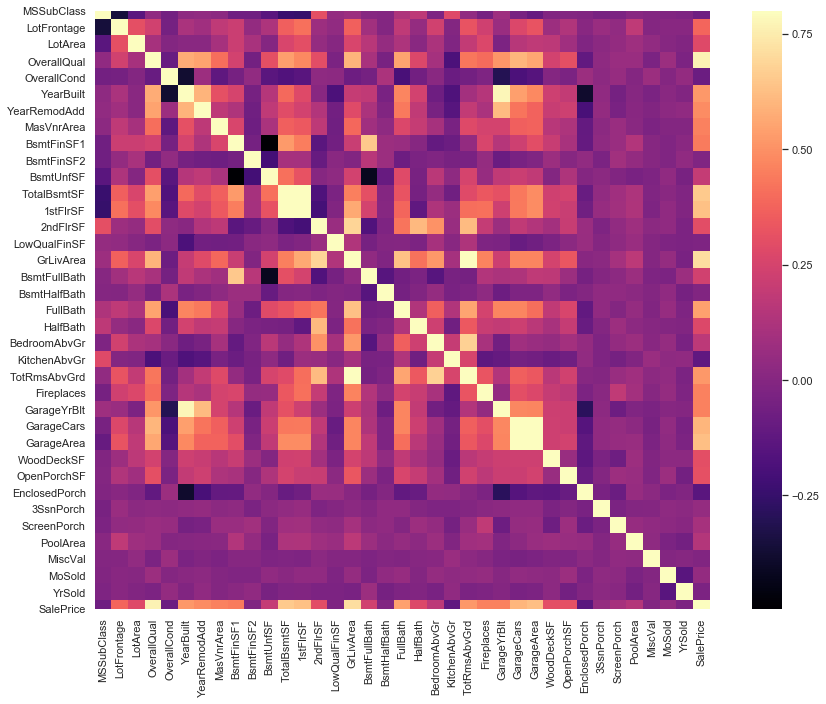
\includegraphics[scale=0.6]{multicoll} 
\end{center}

	Чем светлее ячейка, соответствующая паре признаков $ (feature_i, feature_j) $, тем больше корелляция между ними.
	
	Посмотим значения корелляций в численном виде.
	
\begin{lstlisting}[language=Python][frame=single]
	corr_df = corr.unstack().to_frame().reset_index() 
	#corr.unstack(): сделали двухуровневый индекс, получили series (1 столбец со сложным индексом)
	#reset_index(): превратили индекс в значения ячеек
	new_coor_table = corr_df[corr_df.level_0!=corr_df.level_1].sort_values(0, ascending=False)
	#corr_df.level_0!=corr_df.level_1 : убираем пары с одинаковыми признаками
\end{lstlisting}

	Если есть сильно скоррелированны, то выбросим из каждой пары по одному признаку. Например, хотим выбросить признаки 'TotalBsmtSF', 'GarageYrBlt', 'GarageCars', 'TotRmsAbvGrd', тогда:

\begin{lstlisting}[language=Python][frame=single]
	data.drop(['TotalBsmtSF', 'GarageYrBlt', 'GarageCars', 'TotRmsAbvGrd'], 1, inplace=True)
\end{lstlisting}

	Строим регрессию.
	
\begin{lstlisting}[language=Python][frame=single]
	x = add_constant(data.drop(['SalePrice'], 1))
	y = data['SalePrice']
	ols = OLS(y, x)
	results = ols.fit()
	RSS = results.ssr
	n, k = x.shape[0], x.shape[1]
	sigma2_hat = RSS/(n-k)
\end{lstlisting}

	Проверим остатки на нормальность:
	
\begin{lstlisting}[language=Python][frame=single]
	probplot(stand_residuals, plot=plt);
	sns.boxplot(data=stand_residuals, orient="h");
\end{lstlisting}

\begin{figure}[h]
  \caption{probplot}
  \centering
    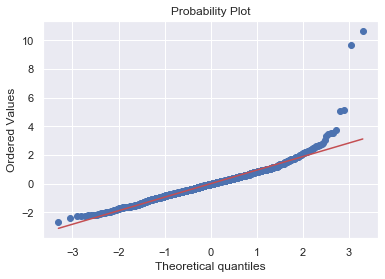
\includegraphics[scale=0.6]{qqplot}
\end{figure}
\begin{figure}[h]
  \caption{boxplot}
  \centering
    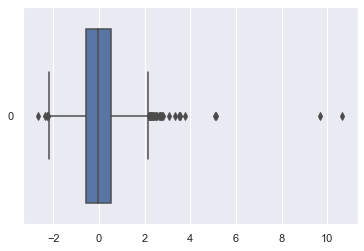
\includegraphics[scale=0.6]{boxplot}
\end{figure}

	Видим, что не очень хорошо все ложится на прямую в случае qqplot, для boxplot есть выбросы $ \Longrightarrow $ есть подозрения на невыаолнение условия нормальности остатков. Разочаруемся в предположении о нормальности до конца:

\begin{lstlisting}[language=Python][frame=single]
	jarque_bera(stand_residuals)
\end{lstlisting}

	Результат : $ Jarque\_beraResult(statistic=16543.863883530954, pvalue=0.0) $, то есть остатки не есть нормальные. Если не хотим применять результаты нормальное регрессии, то это не проблема. Что делать в ином случае? Преобразуем данные: пытаемся брать логорифмы, експоненту и т.д. в надежде на то, что новая реграссия будет удовлетворять условиям нормальности. Можно применить преобразование Бокса - Кокса. Чаще всего используют логарифм.

\begin{lstlisting}[language=Python][frame=single]
	ln_y = np.log(y)
	ln_ols = OLS(ln_y, x)
	ln_results = ln_ols.fit()
	ln_RSS = ln_results.ssr
	n, k = x.shape[0], x.shape[1]
	ln_sigma2_hat = ln_RSS/(n-k)
	ln_influence = ln_results.get_influence()
	ln_residuals = ln_influence.resid
	ln_stand_residuals = ln_residuals/np.sqrt(ln_sigma2_hat)
	probplot(ln_stand_residuals, plot=plt);
	sns.boxplot(data=ln_stand_residuals, orient="h");
	jarque_bera(ln_stand_residuals)
\end{lstlisting}

\begin{figure}[h]
  \caption{probplot}
  \centering
    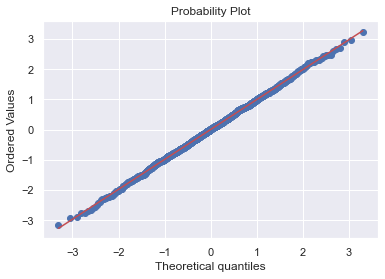
\includegraphics[scale=0.6]{qqplot_ln}
\end{figure}
\begin{figure}[h]
  \caption{boxplot}
  \centering
    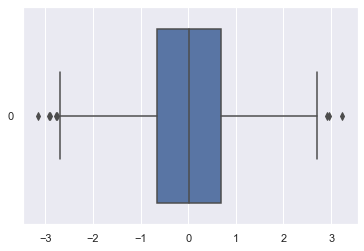
\includegraphics[scale=0.6]{boxplot_ln}
\end{figure}

	Результат теста Харке - Бера: $ Jarque\_beraResult(statistic=0.06510310527385516, pvalue=0.9679725470077343) $, то есть теперь имеем нормальную регрессию.

\begin{remark}
	Помним о том, что мы работаем с логарифмом регрессии, поэтому, когда хотим проводить какие-либо сравнения с исходными данными, необходимо произвести обратное преобразование.
\end{remark}

\section{Отбор признаков. Информационные критерии AIC и BIC}\label{cha:linreg2/sec:otbor+aic+bic}

% \subsection{Отбор признаков.Информационные критерии AIC и BIC.}\label{cha:linreg2}
 
 	Хотим отобрать признаки, для этого нам необходимо сравнивать модели, построенные на разных наборах признаков $ \lbrace x_{i_k} \rbrace_k $ и $ \lbrace x_{i_s} \rbrace_s $. Для этого используются информационные критерии AIC (информационный критерий Акаике) и BIC (Байесовский информационный критерий):
$$\begin{gathered}
  AIC = 2k + n\log(RSS) ,\\
  BIC = \log(n)k + n\log(RSS),
\end{gathered}$$
	где $ RSS = \sum\limits_{i = 1}^n (x_i - \hat{x}_i)^2, \;  \hat{x}_i = z_i\hat{\theta}, \; \hat{\theta} = (Z^TZ)^{-1}Z^TX, \; X = (x_1, \ldots, x_n)$  -- вектор наблюдений, $ Z = (z_{ik}) $ -- матрица факторов (факторов k штук, имеем n наблюдений). Модель с меньшим AIC/BIC - лучшая.
	
\begin{remark}
	Из формулы для подсчета AIC и BIC видно, что BIC штрафует за добавление новых признаков сильнее, чем AIC, поэтому подбор признаков, основанный на BIC, как правило, всегда исключает больше признаков, чем при подборе признаков, основанном на AIC.
\end{remark}

\begin{remark}
	Данные формулы лучше использовать для нормальной регрессии.
\end{remark}
	
\begin{lstlisting}[language=Python][frame=single]
	def select_best_combination(y, x, metric): #metric: 'aic' или 'bic'
    current_factors = x.columns.to_list() #сначала создаем список всех наименований столбцов
    ols = OLS(y, x[current_factors]) 
    results = ols.fit()
    metric_base = getattr(results, metric) 

    while 1 == 1:
        res = pd.Series(index=current_factors) #создаем Series c индексом current_factors и значениями = Nan
        for factor in current_factors:
            ols = OLS(y, x[list(set(current_factors)-{factor})]) #выкидываем по очереди один столбец
            results = ols.fit()
            res.loc[factor] = getattr(results, metric) #вместо Nan в res записываем метрику, соответствующую модели без данного столбца
        res = res.sort_values(ascending=True) #сортируем res по возрастанию 
        if res.iloc[0] < metric_base:
            current_factors.remove(res.index.values[0])
            metric_base = res.iloc[0]
        else:
            break
            
    ols = OLS(y, x[current_factors])
    results = ols.fit()
    
    return current_factors, results
    
    current_factors, results = select_best_combination(ln_y, x, 'bic')
    set(x.columns.to_list()) - set(current_factors) #вывод факторов, основываясь на BIC
    current_factors, results = select_best_combination(ln_y, x, 'aic')
    set(x.columns.to_list()) - set(current_factors) #вывод факторов, основываясь на AIC
\end{lstlisting}

\section{Деление выборки на обучающую и тестовую}\label{cha:linreg2/sec:train+test}

% \subsection{Деление выборки на обучающую и тестовую.}\label{cha:linreg2}

	Разделим выборку на обучающую и тестовую. Разделим случайным образом 75$ \% $ на 25$ \% $:

\begin{lstlisting}[language=Python][frame=single]
	x_train, x_test, y_train, y_test = train_test_split(x, y, test_size=0.25, random_state=10)
\end{lstlisting}

	У моделей из sklearn есть методы fit и predict. fit принимает на вход обучающую выборку и вектор целевых переменных и обучает модель, predict, будучи вызванным после обучения модели, возвращает предсказание на выборке.

\begin{lstlisting}[language=Python][frame=single]
	lr = LinearRegression() #по умолчанию в модели регрессии есть константа
	lr.fit(x_train, y_train)

	y_hat_test = lr.predict(x_test)
	print('Using Y:')
	print('Test MSE %.3f' % mean_squared_error(y_test, y_hat_test))
	print('Test R2 %.3f' % r2_score(y_test, y_hat_test))
	
	y_hat_train = lr.predict(x_train)
	print("Train MSE = %.3f" % mean_squared_error(y_train, y_hat_train))
	print("Train R2 = %.3f" % r2_score(y_train, y_hat_train)) 
\end{lstlisting}

	Вывод:  
	
	Using Y:
	
	Test MSE 1304270005.734
	
	Test R2 0.771
	
	Train MSE = 1342194893.254
	
	Train R2 = 0.813
	
	Если будем использовать логарифмирование данных, получим

\begin{lstlisting}[language=Python][frame=single]
	lr.fit(x_train, np.log(y_train))
	y_hat_test = np.exp(lr.predict(x_test))
	print('Using logY:')
	print('Test MSE %.3f' % mean_squared_error(y_test, y_hat_test))
	print('Test R2 %.3f' % r2_score(y_test, y_hat_test))
\end{lstlisting}

	Вывод:
	
	Using logY:
	
	Test MSE 866920715.293
	
	Test R2 0.848

	Итак, мы обучили модель и посчитали ее качество на тестовой выборке. 

\section{Кросс-валидация}\label{cha:linreg2/sec:crossvalid}

% \subsection{Кросс-валидация.}\label{cha:linreg2}

	Принцип кросс-валидации изображен на рисунке. Берем данные, делим на k групп равного объема (k -- количество фолдов). Делаем все то же самое, что ранее для train и test k раз: для i-го фолда $ i = 1,\ldots,k $ считаем метрику $ metric_i  $ на $ test_i $. Итоговое значение качества модели по кросс - валидации есть значение.
	
$$\begin{gathered} 
\dfrac{\sum\limits_{i =1}^kmetric_i}{k}.
\end{gathered} $$

\begin{figure}[h]
  \caption{5 фолдов}
  \centering
    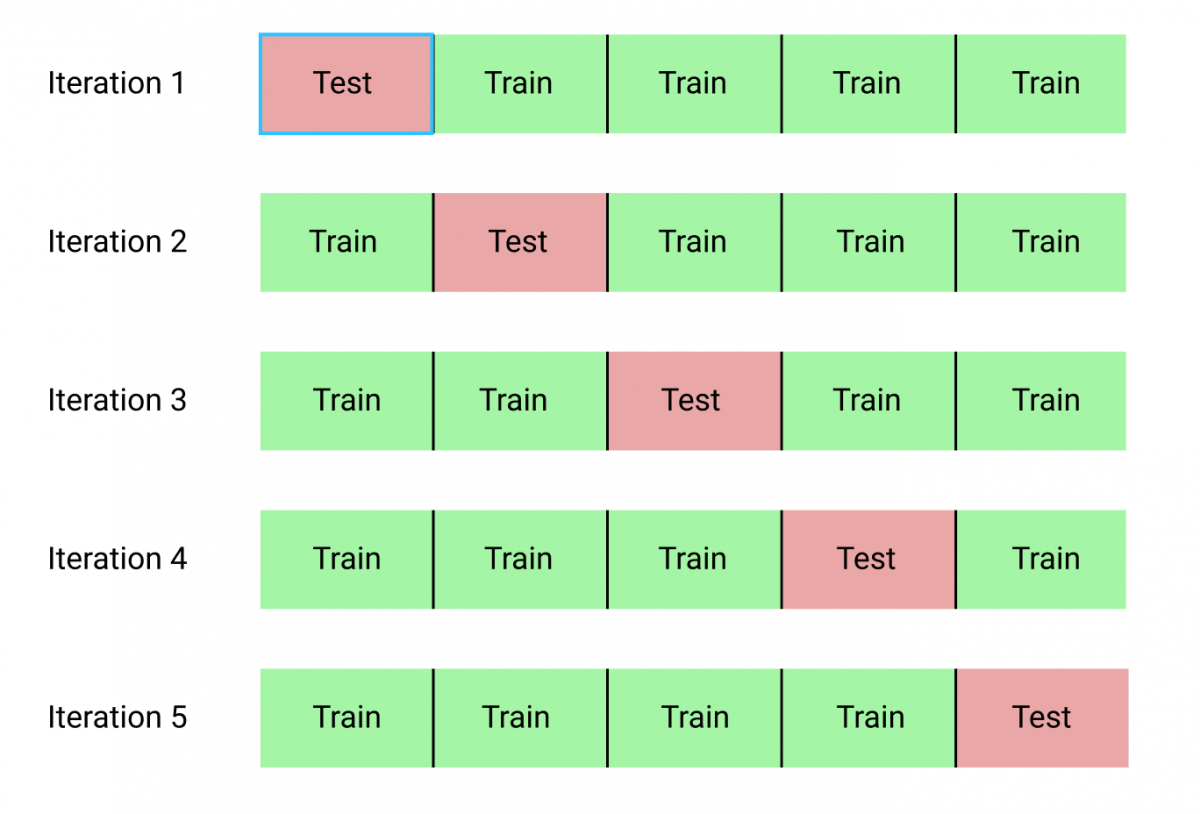
\includegraphics[scale=0.4]{cross_val}
\end{figure}

\begin{lstlisting}[language=Python][frame=single]
	cv_scores = cross_val_score(lr, x, y, cv=10, scoring="neg_mean_squared_error")
\end{lstlisting}

	Если мы выведем $ cv\_scores  $, то результаты получились отрицательными. Это соглашение в sklearn (скоринговую функцию нужно максимизировать). Поэтому все стандартные скореры называются $ neg\_* $, например, $ neg\_mean\_squared\_error  $.
	
\begin{lstlisting}[language=Python][frame=single]
	print("Mean CV MSE = %.4f" % np.mean(-cv_scores)) #итоговое значение качества модели по кросс - валидации
\end{lstlisting}

	В нашем примере она равна Mean CV MSE = 1494450970.6308. Мы всегда можем определить свою метрику и использовать ее, например, в $ cross\_val\_score $. Для этого нужно воспользоваться $ sklearn.metrics.make\_scorer $. Ниже показано, как можно задать свою метрику на примере метрики $ R^2 $ (на самом деле, она прописана в sklearn: $ \# $scoring="r2" в функции $ cross\_val\_score $)
	
\begin{lstlisting}[language=Python][frame=single]
	def r2_squared(y_true, y_pred):
    r2_coef = r2_score(y_true, y_pred)
    return r2_coef

	r2_scorer = make_scorer(r2_squared, greater_is_better=True) #greater_is_better влияет на знаки метрик в cv_scores
	cv_scores = cross_val_score(lr, x, y, cv=10, scoring=r2_scorer) 
	print("Mean CV R2 = %.4f" % np.mean(cv_scores))
	
	cv_scores = cross_val_score(lr, x, ln_y, cv=10, scoring=r2_scorer) 
	print("Mean CV R2 = %.4f" % np.mean(cv_scores))
\end{lstlisting}

	Вывод для не логарифма: Mean CV R2 = 0.7825. Для $ \log y:$  Mean CV R2 = 0.8504.

\subsection{Отбор признаков с помощью кросс-валидации (greedy algorithm)}\label{cha:linreg2/subsec:greedy}

% \subsection{Отбор признаков с помощью кросс-валидации (greedy algorithm).}\label{cha:linreg2}

	Вместо критериев AIC и BIC возьмем итоговое значение качества модели по кросс - валидации:

\begin{lstlisting}[language=Python][frame=single]
def calc_kfold_validation(x, y):
    lr = LinearRegression()
    cv_scores = cross_val_score(lr, x, y, cv=5, scoring="neg_mean_squared_error")
    return np.mean(-cv_scores)
    
def select_best_combination(x, y):
    current_factors = x.columns.to_list() #сначала создаем список всех наименований столбцов
    metric_base = calc_kfold_validation(x[current_factors], y)

    while 1 == 1:
        res = pd.Series(index=current_factors) #создаем Series c индексом current_factors и значениями = Nan
        for factor in current_factors:
            res.loc[factor] = calc_kfold_validation(x[list(set(current_factors)-{factor})], y)
                #вместо Nan в res записываем метрику, соответствующую модели без данного столбца
        res = res.sort_values(ascending=True) #сортируем res по возрастанию 
        if res.iloc[0] < metric_base:
            current_factors.remove(res.index.values[0])
            metric_base = res.iloc[0]
        else:
            break
            
    return current_factors, calc_kfold_validation(x[current_factors], y)
    
 ln_y_train, ln_y_test = np.log(y_train), np.log(y_test)
 current_factors, _ = select_best_combination(x_train, ln_y_train) #делаем отбор признаков на train (по ln_y_train)
 set(x.columns.to_list()) - set(current_factors)
\end{lstlisting}

\subsection*{Сравним модель до и после отбора признаков.}\label{cha:linreg2}

\begin{lstlisting}[language=Python][frame=single]
	k = x_train.shape[1] + 1 #количество факторов (с учетом const)
	n = x_test.shape[0]
	lr = LinearRegression()
	lr.fit(x_train, ln_y_train)

	ln_y_hat_test = lr.predict(x_test)
	print('Test R2 %.3f' % r2_score(ln_y_test, ln_y_hat_test))
	print('Test AIC %.3f' % (2*k + n * np.log(np.sum((ln_y_test - ln_y_hat_test) ** 2))) )
\end{lstlisting}

	Вывод:
	
	Test R2 0.858
	
	Test AIC 835.847

\begin{lstlisting}[language=Python][frame=single]
	k = x_train[current_factors].shape[1] + 1 #количество факторов (с учетом const)
	n = x_test.shape[0]
	lr = LinearRegression()
	lr.fit(x_train[current_factors], ln_y_train)

	ln_y_hat_test = lr.predict(x_test[current_factors])
	print('After greedy algorithm')
	print('Test R2 %.3f' % r2_score(ln_y_test, ln_y_hat_test))
	print('Test AIC %.3f' % (2*k + n * np.log(np.sum((ln_y_test - ln_y_hat_test) ** 2))) )
\end{lstlisting}

	Вывод:
	
	After greedy algorithm
	
	Test R2 0.856
	
	Test AIC 821.092

\section{Гребневая регрессия}\label{cha:linreg2/sec:greb}

Было: $\displaystyle X_i = \theta_1 + Z_{i2}\theta_2 + \dots + Z_{ik} \theta_k + \varepsilon_i = <Z_i, \theta> + \varepsilon_i$.

МНК: $\displaystyle S(\theta) = \left( X - Z \theta \right)^T \left( X - Z \theta \right) \to \underset{\theta}{\min}$.

\begin{theorem}[]\label{lec:greb/the:}
	Если $A = Z^T Z$ не вырождена, то $\exists !$ о.н.к. $\hat{\theta} = \left( Z^T Z \right)^{-1} Z^T X$.
\end{theorem}

Если $A$ необратима, то мы получаем проблему мультиколлинераности, то имеются коррелирующие (линейно зависимые) признаки. Т.е. если $A$ не обратима, то задача $S(\theta) \to \min$ имеет бесконечное число решений, то регрессия получается переобученная.\\
Т.к. $\exists$ линейная зависимость признаков, то $\exists$ вектор $\lambda: \; <Z_i, \lambda> = 0 \; \forall i \; \Rightarrow$
$$\begin{gathered}
	X_i = <\theta, Z_i> + \varepsilon_i \\
	<\hat{\theta} + c \lambda, Z_i> = <\hat{\theta}, Z_i> + c \cdot \underbrace{\sqrt{<\lambda, Z_i>}}_{=0} = <\hat{\theta}, Z_i>
\end{gathered}$$

\section{Регуляризация}\label{cha:linreg2/sec:regul}

Вместо задачи минимизации $S(\theta)$ рассматривается минимизация следующего функицонала:
$$\begin{gathered}
	S_{\alpha} = S(\theta) + \alpha \cdot R(\theta) \to \underset{\theta}{\min} \\
	\text{где } \alpha \text{ - параметр, } R(\theta) \text{ - регуляризатор}
\end{gathered}$$
$L_2: \; R(\theta) = \underset{j=2}{\overset{k}{\sum}}\theta_j^2$ - получаем гребневую регрессию. \\
$L_1: \; R(\theta) = \underset{j=2}{\overset{k}{\sum}}|\theta_j|$.\\

В случае $L_2$ регуляризации $\displaystyle \hat{\theta} = \left( Z^T Z + \alpha \cdot \mathbb{I} \right)^{-1} Z^T X$.

В sklearn есть несколько классов, реализующих линейную регрессию:
\begin{enumerate}
	\item LinearRegression — <<классическая>> линейная регрессия с оптимизацией MSE
	\item Ridge — линейная регрессия с оптимизацией MSE и $l_2$-регуляризацией
	\item Lasso — линейная регрессия с оптимизацией MSE и $l_1$-регуляризацией
\end{enumerate}

\begin{lstlisting}[language=Python]
	lr = LinearRegression()
	lr = Ridge() #по умолчанию alpha=1.0, fit_intercept=True
	lr.fit(x_train, y_train)

	y_hat_test = lr.predict(x_test)
	print('Test MSE %.3f' % mean_squared_error(y_test, y_hat_test))
	print('Test R2 %.3f' % r2_score(y_test, y_hat_test))

	#для сравнения
	y_hat_train = lr.predict(x_train)
	print("Train MSE = %.3f" % mean_squared_error(y_train, y_hat_train))
	print("Train R2 = %.3f" % r2_score(y_train, y_hat_train))
\end{lstlisting}

\section{Отбор признаков}\label{cha:linreg2/sec:otborprizn}

Посмотрим на то, какие признаки оказались самыми "сильными". Для этого визуализируем коэффициенты регрессии, соответствующие признакам.

\begin{lstlisting}[language=Python]
	sorted(zip(a, b, c), reverse=True) #сортировка по 1ым элементам по убыванию

	def show_weights(features, weights, scales):
	    fig, axs = plt.subplots(figsize=(14, 10), ncols=2) #ncols=2: два графика (два столбца)
	    sorted_weights = sorted(zip(weights, features, scales), reverse=True) #сортировка по весам по убыванию
	    weights = [x[0] for x in sorted_weights]
	    features = [x[1] for x in sorted_weights]
	    scales = [x[2] for x in sorted_weights]
	    sns.barplot(y=features, x=weights, ax=axs[0])
	    axs[0].set_xlabel("Weight")
	    sns.barplot(y=features, x=scales, ax=axs[1])
	    axs[1].set_xlabel("Scale")
	    plt.tight_layout()

	show_weights(x_train.columns, lr.coef_, x_train.std())
\end{lstlisting}

Будем масштабировать наши признаки. Это сделает нашу регуляризацию более честной: теперь все признаки будут регуляризоваться в равной степени.

Для этого воспользуемся трансформером StandardScaler. Трансформеры в sklearn имеют методы fit и transform (а еще fittransform). Метод fit принимает на вход обучающую выборку и считает по ней необходимые значения (среднее и стандартное отклонение каждого из признаков). transform применяет преобразование к переданной выборке.

\begin{lstlisting}[language=Python]
	scaler = StandardScaler()
	x_train_scaled = scaler.fit_transform(x_train)
	x_test_scaled = scaler.transform(x_test) #на test делаем только transform!

	lr = Ridge()
	lr.fit(x_train_scaled, y_train)

	show_weights(x_train.columns, lr.coef_, x_train_scaled.std(axis=0)) #type(x_train_scaled
\end{lstlisting}

\section{Подбор гиперпараметров}\label{cha:linreg2/sec:hyperpar}

Наряду с параметрами, которые модель оптимизирует на этапе обучения (коэффициенты регрессии), у модели есть и гиперпараметры. У нашей модели это alpha — коэффициент регуляризации.

Будем пользоваться кросс-валидацией для подбора гиперпараметров.

Подберем alpha по логарифмической сетке, чтобы узнать оптимальный порядок величины.

\begin{lstlisting}[language=Python]
	from sklearn.metrics import make_scorer

	def r2_squared(y_true, y_pred):
	    r2_coef = r2_score(y_true, y_pred)
	    return r2_coef

	r2_scorer = make_scorer(r2_squared, greater_is_better=True)

	alphas = np.logspace(-2, 3, 20)
	searcher = GridSearchCV(Ridge(), [{"alpha": alphas}], scoring=r2_scorer, cv=10) #scoring="r2"
	searcher.fit(x_train_scaled, y_train)

	best_alpha = searcher.best_params_["alpha"]
	print("Best alpha = %.4f" % best_alpha)

	plt.plot(alphas, searcher.cv_results_["mean_test_score"])
	plt.xscale("log")
	plt.xlabel("alpha")
	plt.ylabel("CV score")

	lr = Ridge(best_alpha) 
	lr.fit(x_train_scaled, y_train)

	y_hat_test = lr.predict(x_test_scaled)
	print('Test MSE %.3f' % mean_squared_error(y_test, y_hat_test))
	print('Test R2 %.3f' % r2_score(y_test, y_hat_test))

	lr.intercept_

	lr = Ridge() 
	lr.fit(x_train_scaled, y_train)

	y_hat_test = lr.predict(x_test_scaled)
	print('Test MSE %.3f' % mean_squared_error(y_test, y_hat_test))
	print('Test R2 %.3f' % r2_score(y_test, y_hat_test))

	lr.intercept_ #обратим внимание на то, что константа в регрессии не регуляризуется
\end{lstlisting}

\subsection*{Пример}\label{cha:linreg2/subsec:prob}

\begin{problem}
	В файле <<House-prices-corrected.csv>> представлены характеристики различных домов (стоимость, площадь, количество комнат, год постройки и тп, описание признаков можно найти по ссылке Ames Housing dataset).
	
	Изучить линейную зависимость стоимости домов (SalePrice) от всех остальных показателей.
\end{problem}

\begin{lstlisting}[language=Python]
	#from sklearn.linear_model import LinearRegression
	from sklearn.linear_model import Ridge
	from sklearn.model_selection import train_test_split
	from sklearn.metrics import mean_squared_error, r2_score
	from sklearn.preprocessing import StandardScaler
	from sklearn.model_selection import GridSearchCV

	data = pd.read_csv('House_prices_corrected.csv')
	x = data.drop(['SalePrice'], 1)
	y = data['SalePrice']

	x_train, x_test, y_train, y_test = train_test_split(x, y, test_size=0.2, random_state=10)

	#lr = LinearRegression()
	lr = Ridge() #по умолчанию alpha=1.0, fit_intercept=True
	lr.fit(x_train, y_train)

	y_hat_test = lr.predict(x_test)
	print('Test MSE %.3f' % mean_squared_error(y_test, y_hat_test))
	print('Test R2 %.3f' % r2_score(y_test, y_hat_test))

	#для сравнения
	y_hat_train = lr.predict(x_train)
	print("Train MSE = %.3f" % mean_squared_error(y_train, y_hat_train))
	print("Train R2 = %.3f" % r2_score(y_train, y_hat_train))
\end{lstlisting}


\chapter{Список возможных importов}\label{cha:import}

\green{import numpy as np}

\green{import scipy as sp}

\green{import pandas as pd}

\green{import scipy.stats as st}

\green{import scikit$\_$posthocs as sp} (post hoc tests)

\green{import pingouin as pg}

\green{from scipy.stats import norm} (нормальное распределение)

\green{from scipy.stats import uniform} (равномерное распределение)

\green{from scipy.stats import expon} (экспоненциальное распределение)

\green{from scipy.stats import beta} (бета-распределение)

\green{from scipy.stats import cauchy} (распределение Коши)

\green{from scipy.stats import t} (распределение Стьюдента)

\green{from scipy.stats import f} (распределение Фишера)

\green{from scipy.stats import chi2} (распределение хи-квадрат)

\green{from scipy.stats import gamma} (гамма распределение)

\green{from scipy.stats import binom} (биномиальное распределение)

\green{from scipy.stats import ttest$\_$1samp} (t-test 1 sample)

\green{from scipy.stats import ttest$\_$rel} (t-test для парных выборок)

\green{from scipy.stats import ttest$\_$ind} (t-test с поправкой на неравенство дисперсий)

\green{from scipy.stats import binom$\_$test} (биномильный критерий)

\green{from scipy.stats import wilcoxon} (знако-ранговый критерий Вилкоксона)

\green{from statsmodels.stats.diagnostic import lilliefors} (тест Лиллиефорса)

\green{from scipy.stats import mannwhitneyu} (критерий Манна и Уитни)

\green{from scipy.stats import ks$\_$2samp} (критерий Смирного)

\green{from scipy.stats import anderson$\_$ksamp} (критерий Андерсона-Дарлинга)

\green{from scipy.stats import kruskal} (критерий Краскела-Уоллиса)

\green{from scipy.stats import bartlett} (критерий Бартлетта)

\green{from scipy.stats import f$\_$oneway} (ANOVA)

\green{from scipy.stats import friedmanchisquare} (критерий Фридмана)

\green{from statsmodels.stats.anova import AnovaRM} (критерий Фишера aka ANOVA RM)

\green{} ()

\green{} ()

\green{} ()

\green{} ()

\green{} ()


\cleardoublepage
\phantomsection
\addcontentsline{toc}{chapter}{Список используемой литературы}
\begin{thebibliography}{}
	\bibitem{0}
		Курс лекций И.М.Никонова, механико-математический факультет МГУ им. М.В.Ломоносова, 2021 г.
	\bibitem{1}
		Курс семинаров И.М.Никонова, механико-математический факультет МГУ им. М.В.Ломоносова, 2021 г.
\end{thebibliography}

\end{document}
